% Options for packages loaded elsewhere
\PassOptionsToPackage{unicode}{hyperref}
\PassOptionsToPackage{hyphens}{url}
\PassOptionsToPackage{dvipsnames,svgnames,x11names}{xcolor}
%
\documentclass[
  10pt,
  letterpaper,
  DIV=11,
  numbers=noendperiod]{scrreprt}

\usepackage{amsmath,amssymb}
\usepackage{setspace}
\usepackage{iftex}
\ifPDFTeX
  \usepackage[T1]{fontenc}
  \usepackage[utf8]{inputenc}
  \usepackage{textcomp} % provide euro and other symbols
\else % if luatex or xetex
  \usepackage{unicode-math}
  \defaultfontfeatures{Scale=MatchLowercase}
  \defaultfontfeatures[\rmfamily]{Ligatures=TeX,Scale=1}
\fi
\usepackage{lmodern}
\ifPDFTeX\else  
    % xetex/luatex font selection
  \setmainfont[]{Verdana}
  \setmonofont[]{Lucida Sans Typewriter}
  \setmathfont[]{Arial}
\fi
% Use upquote if available, for straight quotes in verbatim environments
\IfFileExists{upquote.sty}{\usepackage{upquote}}{}
\IfFileExists{microtype.sty}{% use microtype if available
  \usepackage[]{microtype}
  \UseMicrotypeSet[protrusion]{basicmath} % disable protrusion for tt fonts
}{}
\usepackage{xcolor}
\usepackage[margin = 1in]{geometry}
\setlength{\emergencystretch}{3em} % prevent overfull lines
\setcounter{secnumdepth}{3}
% Make \paragraph and \subparagraph free-standing
\ifx\paragraph\undefined\else
  \let\oldparagraph\paragraph
  \renewcommand{\paragraph}[1]{\oldparagraph{#1}\mbox{}}
\fi
\ifx\subparagraph\undefined\else
  \let\oldsubparagraph\subparagraph
  \renewcommand{\subparagraph}[1]{\oldsubparagraph{#1}\mbox{}}
\fi

\usepackage{color}
\usepackage{fancyvrb}
\newcommand{\VerbBar}{|}
\newcommand{\VERB}{\Verb[commandchars=\\\{\}]}
\DefineVerbatimEnvironment{Highlighting}{Verbatim}{commandchars=\\\{\}}
% Add ',fontsize=\small' for more characters per line
\usepackage{framed}
\definecolor{shadecolor}{RGB}{241,243,245}
\newenvironment{Shaded}{\begin{snugshade}}{\end{snugshade}}
\newcommand{\AlertTok}[1]{\textcolor[rgb]{0.68,0.00,0.00}{#1}}
\newcommand{\AnnotationTok}[1]{\textcolor[rgb]{0.37,0.37,0.37}{#1}}
\newcommand{\AttributeTok}[1]{\textcolor[rgb]{0.40,0.45,0.13}{#1}}
\newcommand{\BaseNTok}[1]{\textcolor[rgb]{0.68,0.00,0.00}{#1}}
\newcommand{\BuiltInTok}[1]{\textcolor[rgb]{0.00,0.23,0.31}{#1}}
\newcommand{\CharTok}[1]{\textcolor[rgb]{0.13,0.47,0.30}{#1}}
\newcommand{\CommentTok}[1]{\textcolor[rgb]{0.37,0.37,0.37}{#1}}
\newcommand{\CommentVarTok}[1]{\textcolor[rgb]{0.37,0.37,0.37}{\textit{#1}}}
\newcommand{\ConstantTok}[1]{\textcolor[rgb]{0.56,0.35,0.01}{#1}}
\newcommand{\ControlFlowTok}[1]{\textcolor[rgb]{0.00,0.23,0.31}{#1}}
\newcommand{\DataTypeTok}[1]{\textcolor[rgb]{0.68,0.00,0.00}{#1}}
\newcommand{\DecValTok}[1]{\textcolor[rgb]{0.68,0.00,0.00}{#1}}
\newcommand{\DocumentationTok}[1]{\textcolor[rgb]{0.37,0.37,0.37}{\textit{#1}}}
\newcommand{\ErrorTok}[1]{\textcolor[rgb]{0.68,0.00,0.00}{#1}}
\newcommand{\ExtensionTok}[1]{\textcolor[rgb]{0.00,0.23,0.31}{#1}}
\newcommand{\FloatTok}[1]{\textcolor[rgb]{0.68,0.00,0.00}{#1}}
\newcommand{\FunctionTok}[1]{\textcolor[rgb]{0.28,0.35,0.67}{#1}}
\newcommand{\ImportTok}[1]{\textcolor[rgb]{0.00,0.46,0.62}{#1}}
\newcommand{\InformationTok}[1]{\textcolor[rgb]{0.37,0.37,0.37}{#1}}
\newcommand{\KeywordTok}[1]{\textcolor[rgb]{0.00,0.23,0.31}{#1}}
\newcommand{\NormalTok}[1]{\textcolor[rgb]{0.00,0.23,0.31}{#1}}
\newcommand{\OperatorTok}[1]{\textcolor[rgb]{0.37,0.37,0.37}{#1}}
\newcommand{\OtherTok}[1]{\textcolor[rgb]{0.00,0.23,0.31}{#1}}
\newcommand{\PreprocessorTok}[1]{\textcolor[rgb]{0.68,0.00,0.00}{#1}}
\newcommand{\RegionMarkerTok}[1]{\textcolor[rgb]{0.00,0.23,0.31}{#1}}
\newcommand{\SpecialCharTok}[1]{\textcolor[rgb]{0.37,0.37,0.37}{#1}}
\newcommand{\SpecialStringTok}[1]{\textcolor[rgb]{0.13,0.47,0.30}{#1}}
\newcommand{\StringTok}[1]{\textcolor[rgb]{0.13,0.47,0.30}{#1}}
\newcommand{\VariableTok}[1]{\textcolor[rgb]{0.07,0.07,0.07}{#1}}
\newcommand{\VerbatimStringTok}[1]{\textcolor[rgb]{0.13,0.47,0.30}{#1}}
\newcommand{\WarningTok}[1]{\textcolor[rgb]{0.37,0.37,0.37}{\textit{#1}}}

\providecommand{\tightlist}{%
  \setlength{\itemsep}{0pt}\setlength{\parskip}{0pt}}\usepackage{longtable,booktabs,array}
\usepackage{calc} % for calculating minipage widths
% Correct order of tables after \paragraph or \subparagraph
\usepackage{etoolbox}
\makeatletter
\patchcmd\longtable{\par}{\if@noskipsec\mbox{}\fi\par}{}{}
\makeatother
% Allow footnotes in longtable head/foot
\IfFileExists{footnotehyper.sty}{\usepackage{footnotehyper}}{\usepackage{footnote}}
\makesavenoteenv{longtable}
\usepackage{graphicx}
\makeatletter
\def\maxwidth{\ifdim\Gin@nat@width>\linewidth\linewidth\else\Gin@nat@width\fi}
\def\maxheight{\ifdim\Gin@nat@height>\textheight\textheight\else\Gin@nat@height\fi}
\makeatother
% Scale images if necessary, so that they will not overflow the page
% margins by default, and it is still possible to overwrite the defaults
% using explicit options in \includegraphics[width, height, ...]{}
\setkeys{Gin}{width=\maxwidth,height=\maxheight,keepaspectratio}
% Set default figure placement to htbp
\makeatletter
\def\fps@figure{htbp}
\makeatother

\usepackage{booktabs}
\usepackage{longtable}
\usepackage{array}
\usepackage{multirow}
\usepackage{wrapfig}
\usepackage{float}
\usepackage{colortbl}
\usepackage{pdflscape}
\usepackage{tabu}
\usepackage{threeparttable}
\usepackage{threeparttablex}
\usepackage[normalem]{ulem}
\usepackage{makecell}
\usepackage{xcolor}
\KOMAoption{captions}{tableheading}
\makeatletter
\makeatother
\makeatletter
\makeatother
\makeatletter
\@ifpackageloaded{caption}{}{\usepackage{caption}}
\AtBeginDocument{%
\ifdefined\contentsname
  \renewcommand*\contentsname{Tabla de contenidos}
\else
  \newcommand\contentsname{Tabla de contenidos}
\fi
\ifdefined\listfigurename
  \renewcommand*\listfigurename{Listado de figuras}
\else
  \newcommand\listfigurename{Listado de figuras}
\fi
\ifdefined\listtablename
  \renewcommand*\listtablename{Listado de Tablas}
\else
  \newcommand\listtablename{Listado de Tablas}
\fi
\ifdefined\figurename
  \renewcommand*\figurename{Figura}
\else
  \newcommand\figurename{Figura}
\fi
\ifdefined\tablename
  \renewcommand*\tablename{Tabla}
\else
  \newcommand\tablename{Tabla}
\fi
}
\@ifpackageloaded{float}{}{\usepackage{float}}
\floatstyle{ruled}
\@ifundefined{c@chapter}{\newfloat{codelisting}{h}{lop}}{\newfloat{codelisting}{h}{lop}[chapter]}
\floatname{codelisting}{Listado}
\newcommand*\listoflistings{\listof{codelisting}{Listado de Listados}}
\makeatother
\makeatletter
\@ifpackageloaded{caption}{}{\usepackage{caption}}
\@ifpackageloaded{subcaption}{}{\usepackage{subcaption}}
\makeatother
\makeatletter
\@ifpackageloaded{tcolorbox}{}{\usepackage[skins,breakable]{tcolorbox}}
\makeatother
\makeatletter
\@ifundefined{shadecolor}{\definecolor{shadecolor}{rgb}{.97, .97, .97}}
\makeatother
\makeatletter
\makeatother
\makeatletter
\makeatother
\ifLuaTeX
\usepackage[bidi=basic]{babel}
\else
\usepackage[bidi=default]{babel}
\fi
\babelprovide[main,import]{spanish}
% get rid of language-specific shorthands (see #6817):
\let\LanguageShortHands\languageshorthands
\def\languageshorthands#1{}
\ifLuaTeX
  \usepackage{selnolig}  % disable illegal ligatures
\fi
\usepackage[style=authoryear,]{biblatex}
\addbibresource{references.bib}
\IfFileExists{bookmark.sty}{\usepackage{bookmark}}{\usepackage{hyperref}}
\IfFileExists{xurl.sty}{\usepackage{xurl}}{} % add URL line breaks if available
\urlstyle{same} % disable monospaced font for URLs
\hypersetup{
  pdftitle={ANÁLISIS MULTIVARIANTE PARA COMPARAR EL ESTADO ECOLÓGICO DE LAS COMUNIDADES DE MACROINVERTEBRADOS EN RÍOS DEL PÁRAMO ECUATORIANO Y SU IMPACTO EN ÁREAS DE CONSERVACIÓN},
  pdfauthor={Karina Hernández},
  pdflang={es},
  colorlinks=true,
  linkcolor={black},
  filecolor={Maroon},
  citecolor={Blue},
  urlcolor={cyan},
  pdfcreator={LaTeX via pandoc}}

\title{ANÁLISIS MULTIVARIANTE PARA COMPARAR EL ESTADO ECOLÓGICO DE LAS
COMUNIDADES DE MACROINVERTEBRADOS EN RÍOS DEL PÁRAMO ECUATORIANO Y SU
IMPACTO EN ÁREAS DE CONSERVACIÓN\thanks{MAESTRÍA EN BIODIVERSIDAD Y
CAMBIO CLIMÁTICO}}
\usepackage{etoolbox}
\makeatletter
\providecommand{\subtitle}[1]{% add subtitle to \maketitle
  \apptocmd{\@title}{\par {\large #1 \par}}{}{}
}
\makeatother
\subtitle{Maestría en Biodiversidad y Cambio Climático}
\author{Karina Hernández}
\date{16 de abril de 2024}

\begin{document}
\maketitle
\begin{abstract}
En el presente Notebook de RMarkdown, se desarrolla todo el proceso
estadístico multivariante que busca Analizar las Componentes Principales
(ACP) y los Clúster que determinan la taxonomía de variables que
identifican de mejor forma a las comunidades de macroinvertebrados en
ríos del páramo ecuatoriano. Primero, se aplicará un ACP para reducir la
dimensionalidad de los datos y examinar patrones de variación en la
composición de las variables físico-quimicas y ecológicas entre
diferentes ríos. Se realizará una evaluación de la adecuación del modelo
mediante el estadístico de Kaiser-Meyer-Olkin (KMO) con su nivel
significancia respecto al Test de Bartlett, el cual nos proporcionará
información sobre la idoneidad de los datos para la aplicación del
componentes principales. Además, se empleará un algoritmo de Clúster
para agrupar variables en función de su similitud, esto permitirá
identificar patrones para definir grupo de variables y xplorar posibles
diferencias. Al integrar estos enfoques analíticos, este estudio busca
proporcionar una comprensión más profunda del estado ecológico de los
ríos del páramo ecuatoriano y de la efectividad de las áreas de
conservación en la protección de las comunidades de macroinvertebrados.
Los hallazgos de este análisis contribuirán a informar futuras
estrategias de conservación y gestión de estos ecosistemas críticos.
\end{abstract}
\ifdefined\Shaded\renewenvironment{Shaded}{\begin{tcolorbox}[enhanced, frame hidden, interior hidden, boxrule=0pt, borderline west={3pt}{0pt}{shadecolor}, sharp corners, breakable]}{\end{tcolorbox}}\fi

\renewcommand*\contentsname{\textbf{CONTENIDOS}}
{
\hypersetup{linkcolor=green}
\setcounter{tocdepth}{2}
\tableofcontents
}
\listoffigures
\listoftables
\setstretch{1.5}
\begin{Shaded}
\begin{Highlighting}[numbers=left,,]
\CommentTok{\# Librerías y directorio de trabajo:}
\FunctionTok{library}\NormalTok{(tidyverse)}
\FunctionTok{library}\NormalTok{(DT)}
\FunctionTok{library}\NormalTok{(highcharter)}
\FunctionTok{library}\NormalTok{(psych)}
\FunctionTok{library}\NormalTok{(gridExtra)}
\FunctionTok{library}\NormalTok{(glue)}
\FunctionTok{library}\NormalTok{(e1071)}
\FunctionTok{library}\NormalTok{(reshape2)}
\FunctionTok{library}\NormalTok{(factoextra)}
\FunctionTok{library}\NormalTok{(FactoMineR)}
\FunctionTok{library}\NormalTok{(corrplot)}
\FunctionTok{library}\NormalTok{(knitr)}
\FunctionTok{library}\NormalTok{(kableExtra)}
\FunctionTok{library}\NormalTok{(RColorBrewer) }\CommentTok{\# Librería para la paleta de colores}

\NormalTok{knitr}\SpecialCharTok{::}\NormalTok{opts\_knit}\SpecialCharTok{$}\FunctionTok{set}\NormalTok{(}\AttributeTok{root.dir =} \StringTok{"C:/Users/marcelochavez/Documents/TESIS/KARINA/"}\NormalTok{)}
\end{Highlighting}
\end{Shaded}

\hypertarget{anuxe1lisis-exploratorio-de-los-uxedndices-fuxedsquico-quuxedmicos-y-ecoluxf3gicos}{%
\chapter{Análisis Exploratorio de los Índices Físquico-Químicos y
Ecológicos}\label{anuxe1lisis-exploratorio-de-los-uxedndices-fuxedsquico-quuxedmicos-y-ecoluxf3gicos}}

Empezaremos con mostrar un Boxplot comparativo para visualizar si
existen valores atípicos y como se distribuyen las variables en los años
\textbf{1995 y 2021} según el formato o estructura de cada tabla con
escalas de medición orignales en cada variable:

\hypertarget{dataset-de-los-uxedndices-fuxedsico-quuxedmicos}{%
\section{Dataset de los Índices Físico
Químicos:}\label{dataset-de-los-uxedndices-fuxedsico-quuxedmicos}}

\begin{Shaded}
\begin{Highlighting}[numbers=left,,]
\CommentTok{\# Carga del DataSet y transformaciones {-}{-}{-}{-}{-}{-}{-}{-}{-}{-}{-}{-}{-}{-}{-}{-}{-}{-}{-}{-}{-}{-}{-}{-}{-}{-}{-}{-}{-}{-}{-}{-}{-}{-}{-}{-}{-}{-}{-}{-}{-}}

\NormalTok{indices\_fq }\OtherTok{\textless{}{-}}\NormalTok{ readxl}\SpecialCharTok{::}\FunctionTok{read\_excel}\NormalTok{(}\StringTok{"DATASETS/DatosFisicoQuimicosEcologicos.xlsx"}\NormalTok{) }\SpecialCharTok{\%\textgreater{}\%} 
  \FunctionTok{mutate\_if}\NormalTok{(is.numeric, }\SpecialCharTok{\textasciitilde{}} \FunctionTok{round}\NormalTok{(., }\DecValTok{2}\NormalTok{)) }\SpecialCharTok{\%\textgreater{}\%}
  \FunctionTok{rename\_all}\NormalTok{(toupper)}

\NormalTok{df\_largo }\OtherTok{\textless{}{-}}\NormalTok{ indices\_fq }\SpecialCharTok{\%\textgreater{}\%}
    \FunctionTok{pivot\_longer}\NormalTok{(}\AttributeTok{cols =} \SpecialCharTok{{-}}\NormalTok{RIOS, }
                 \AttributeTok{names\_to =} \FunctionTok{c}\NormalTok{(}\StringTok{".value"}\NormalTok{, }\StringTok{"ANIO"}\NormalTok{), }
                 \AttributeTok{names\_pattern =} \StringTok{"(.*)\_(}\SpecialCharTok{\textbackslash{}\textbackslash{}}\StringTok{d\{4\})"}\NormalTok{)}

\NormalTok{indices\_fq\_ddc }\OtherTok{\textless{}{-}}\NormalTok{ df\_largo }\SpecialCharTok{\%\textgreater{}\%}
    \FunctionTok{mutate}\NormalTok{(}\AttributeTok{ID =} \FunctionTok{glue}\NormalTok{(}\StringTok{"\{RIOS\}\_\{ANIO\}"}\NormalTok{)) }\SpecialCharTok{\%\textgreater{}\%}
    \FunctionTok{column\_to\_rownames}\NormalTok{(}\AttributeTok{var =} \StringTok{"ID"}\NormalTok{) }\SpecialCharTok{\%\textgreater{}\%} 
    \FunctionTok{select}\NormalTok{(}\SpecialCharTok{{-}}\NormalTok{RIOS,}
           \SpecialCharTok{{-}}\NormalTok{ANIO)}

\NormalTok{var\_scale }\OtherTok{\textless{}{-}} \FunctionTok{as.data.frame}\NormalTok{(}\FunctionTok{lapply}\NormalTok{(indices\_fq\_ddc, }\ControlFlowTok{function}\NormalTok{(x) }\ControlFlowTok{if}\NormalTok{(}\FunctionTok{is.numeric}\NormalTok{(x)) }\FunctionTok{scale}\NormalTok{(x) }\ControlFlowTok{else}\NormalTok{ x))}

\NormalTok{df\_fq\_1995 }\OtherTok{\textless{}{-}} \FunctionTok{pivot\_longer}\NormalTok{(df\_largo,}
                                \AttributeTok{cols =} \FunctionTok{c}\NormalTok{(ANCHO,}
\NormalTok{                                         PROFUNDIDAD,}
\NormalTok{                                         VELOCIDAD,}
\NormalTok{                                         DESCARGA,}
\NormalTok{                                         PH,}
\NormalTok{                                         TEMPERATURA,}
\NormalTok{                                         OXIGENO\_DISUELTO,}
\NormalTok{                                         CONDUCTIVIDAD,}
\NormalTok{                                         RIQUEZA,}
\NormalTok{                                         ABUNDANCIA,}
\NormalTok{                                         DIVERSIDAD,}
\NormalTok{                                         ABI,}
\NormalTok{                                         BMWP,}
\NormalTok{                                         IBF),}
                                \AttributeTok{names\_to =} \StringTok{"VARIABLE"}\NormalTok{,}
                                \AttributeTok{values\_to =} \StringTok{"VALOR"}\NormalTok{) }\SpecialCharTok{\%\textgreater{}\%} 
    \FunctionTok{filter}\NormalTok{(ANIO}\SpecialCharTok{==}\StringTok{"1995"}\NormalTok{)}

\NormalTok{df\_fq\_2021 }\OtherTok{\textless{}{-}} \FunctionTok{pivot\_longer}\NormalTok{(df\_largo, }
                           \AttributeTok{cols =} \FunctionTok{c}\NormalTok{(ANCHO,}
\NormalTok{                                    PROFUNDIDAD,}
\NormalTok{                                    VELOCIDAD,}
\NormalTok{                                    DESCARGA,}
\NormalTok{                                    PH,}
\NormalTok{                                    TEMPERATURA,}
\NormalTok{                                    OXIGENO\_DISUELTO,}
\NormalTok{                                    CONDUCTIVIDAD,}
\NormalTok{                                    RIQUEZA,}
\NormalTok{                                    ABUNDANCIA,}
\NormalTok{                                    DIVERSIDAD,}
\NormalTok{                                    ABI,}
\NormalTok{                                    BMWP,}
\NormalTok{                                    IBF),}
                           \AttributeTok{names\_to =} \StringTok{"VARIABLE"}\NormalTok{,}
                           \AttributeTok{values\_to =} \StringTok{"VALOR"}\NormalTok{) }\SpecialCharTok{\%\textgreater{}\%} 
    \FunctionTok{filter}\NormalTok{(ANIO}\SpecialCharTok{==}\StringTok{"2021"}\NormalTok{)}


\CommentTok{\# Data para BoxPlot:}

\NormalTok{df\_bx\_95 }\OtherTok{\textless{}{-}} \FunctionTok{data\_to\_boxplot}\NormalTok{(}
\NormalTok{    df\_fq\_1995,}
    \AttributeTok{variable =}\NormalTok{ VALOR,}
    \AttributeTok{group\_var =}\NormalTok{ VARIABLE,}
    \CommentTok{\# group\_var2 = codigo,}
    \AttributeTok{add\_outliers =}\NormalTok{ T}
\NormalTok{)}

\NormalTok{df\_bx\_21 }\OtherTok{\textless{}{-}} \FunctionTok{data\_to\_boxplot}\NormalTok{(}
\NormalTok{    df\_fq\_2021,}
    \AttributeTok{variable =}\NormalTok{ VALOR,}
    \AttributeTok{group\_var =}\NormalTok{ VARIABLE,}
    \CommentTok{\# group\_var2 = codigo,}
    \AttributeTok{add\_outliers =}\NormalTok{ T}
\NormalTok{)}

\CommentTok{\# Visualización del Dataset}

\NormalTok{DT}\SpecialCharTok{::}\FunctionTok{datatable}\NormalTok{(df\_largo,}
              \AttributeTok{class =} \StringTok{\textquotesingle{}cell{-}border stripe\textquotesingle{}}\NormalTok{,}
              \CommentTok{\# filter = \textquotesingle{}top\textquotesingle{},}
              \AttributeTok{caption =}\NormalTok{ htmltools}\SpecialCharTok{::}\NormalTok{tags}\SpecialCharTok{$}\FunctionTok{caption}\NormalTok{(}
              \AttributeTok{style =} \StringTok{\textquotesingle{}caption{-}side: bottom; text{-}align: left;\textquotesingle{}}\NormalTok{,}
              \StringTok{\textquotesingle{}Tabla 1: \textquotesingle{}}\NormalTok{, htmltools}\SpecialCharTok{::}\FunctionTok{em}\NormalTok{(}\StringTok{\textquotesingle{}Indicadores Físico{-}Químicos y Ecológicos para los años 1995 y 2021\textquotesingle{}}\NormalTok{)),}
              \AttributeTok{extensions =} \FunctionTok{c}\NormalTok{(}\StringTok{\textquotesingle{}Buttons\textquotesingle{}}\NormalTok{,}\StringTok{\textquotesingle{}Scroller\textquotesingle{}}\NormalTok{),}
              \AttributeTok{options =} \FunctionTok{list}\NormalTok{(}\AttributeTok{scrollX =} \ConstantTok{TRUE}\NormalTok{,}
                             \AttributeTok{initComplete =} \FunctionTok{JS}\NormalTok{(}
    \StringTok{"function(settings, json) \{"}\NormalTok{,}
    \StringTok{"$(this.api().table().header()).css(\{\textquotesingle{}background{-}color\textquotesingle{}: \textquotesingle{}\#000\textquotesingle{}, \textquotesingle{}color\textquotesingle{}: \textquotesingle{}\#fff\textquotesingle{}\});"}\NormalTok{,}
    \StringTok{"\}"}\NormalTok{),}
    \AttributeTok{dom =} \StringTok{\textquotesingle{}Bfrtip\textquotesingle{}}\NormalTok{,}
    \AttributeTok{buttons =} \FunctionTok{c}\NormalTok{(}\StringTok{\textquotesingle{}excel\textquotesingle{}}\NormalTok{),}
    \AttributeTok{deferRender =} \ConstantTok{TRUE}\NormalTok{,}
    \AttributeTok{scrollY =} \DecValTok{500}\NormalTok{,}
    \AttributeTok{scroller =} \ConstantTok{TRUE}\NormalTok{))}
\end{Highlighting}
\end{Shaded}

\hypertarget{boxplot-de-los-indicadores-fuxedsico-quuxedmicos-y-ecoluxf3gicos}{%
\section{Boxplot de los indicadores físico-químicos y
ecológicos:}\label{boxplot-de-los-indicadores-fuxedsico-quuxedmicos-y-ecoluxf3gicos}}

\begin{Shaded}
\begin{Highlighting}[numbers=left,,]
\FunctionTok{highchart}\NormalTok{() }\SpecialCharTok{\%\textgreater{}\%}
    \FunctionTok{hc\_xAxis}\NormalTok{(}\AttributeTok{type =} \StringTok{"category"}\NormalTok{,}
             \AttributeTok{labels =} \FunctionTok{list}\NormalTok{(}
                 \AttributeTok{rotation =} \DecValTok{270}
\NormalTok{             )) }\SpecialCharTok{\%\textgreater{}\%}
    \FunctionTok{hc\_add\_series\_list}\NormalTok{(df\_bx\_95) }\SpecialCharTok{\%\textgreater{}\%}
    \FunctionTok{hc\_xAxis}\NormalTok{(}\AttributeTok{title =} \FunctionTok{list}\NormalTok{(}\AttributeTok{text =} \StringTok{"VARIABLES"}\NormalTok{)) }\SpecialCharTok{\%\textgreater{}\%}
    \FunctionTok{hc\_yAxis}\NormalTok{(}\AttributeTok{title =} \FunctionTok{list}\NormalTok{(}\AttributeTok{text =} \StringTok{"VALORES"}\NormalTok{)) }\SpecialCharTok{\%\textgreater{}\%}
    \FunctionTok{hc\_title}\NormalTok{(}\AttributeTok{text =} \StringTok{"BOXPLOT COMPARATIVO ENTRE ÍNDICES FÍSICO QUÍMICOS y ECOLÓGICOS {-} AÑO 1995"}\NormalTok{) }\SpecialCharTok{\%\textgreater{}\%}
    \FunctionTok{hc\_subtitle}\NormalTok{(}\AttributeTok{text =} \StringTok{"AÑO 1995"}\NormalTok{, }\AttributeTok{align=}\StringTok{"left"}\NormalTok{) }\SpecialCharTok{\%\textgreater{}\%}
    \FunctionTok{hc\_caption}\NormalTok{(}\AttributeTok{text =} \StringTok{"ELABORADO POR: Karina Hernández"}\NormalTok{) }\SpecialCharTok{\%\textgreater{}\%}
    \FunctionTok{hc\_legend}\NormalTok{(}\AttributeTok{enabled =}\NormalTok{ F, }\AttributeTok{title =} \FunctionTok{list}\NormalTok{(}\AttributeTok{text =} \StringTok{"\textless{}b\textgreater{}ESTACIONES DE MONITOREO:\textless{}/b\textgreater{}"}\NormalTok{)) }\SpecialCharTok{\%\textgreater{}\%}
    \FunctionTok{hc\_tooltip}\NormalTok{(}\AttributeTok{formatter =} \FunctionTok{JS}\NormalTok{(}\StringTok{"function() \{}
\StringTok{    var tooltip = \textquotesingle{}\textquotesingle{};}
\StringTok{    if (this.point.low \&\& this.point.q1 \&\& this.point.median \&\& this.point.q3 \&\& this.point.high) \{}
\StringTok{        tooltip += \textquotesingle{}\textless{}b\textgreater{}Variable: \textless{}/b\textgreater{}\textquotesingle{} + this.point.name + \textquotesingle{}\textless{}br/\textgreater{}\textquotesingle{} +}
\StringTok{                   \textquotesingle{}\textless{}b\textgreater{}Mínimo: \textless{}/b\textgreater{}\textquotesingle{} + this.point.low.toFixed(2) + \textquotesingle{}\textless{}/b\textgreater{}\textless{}br/\textgreater{}\textquotesingle{} +}
\StringTok{                   \textquotesingle{}\textless{}b\textgreater{}Q1: \textless{}/b\textgreater{}\textquotesingle{} + this.point.q1.toFixed(2) + \textquotesingle{}\textless{}/b\textgreater{}\textless{}br/\textgreater{}\textquotesingle{} +}
\StringTok{                   \textquotesingle{}\textless{}b\textgreater{}Mediana: \textless{}/b\textgreater{}\textquotesingle{} + this.point.median.toFixed(2) + \textquotesingle{}\textless{}/b\textgreater{}\textless{}br/\textgreater{}\textquotesingle{} +}
\StringTok{                   \textquotesingle{}\textless{}b\textgreater{}Q3: \textless{}/b\textgreater{}\textquotesingle{} + this.point.q3.toFixed(2) + \textquotesingle{}\textless{}/b\textgreater{}\textless{}br/\textgreater{}\textquotesingle{} +}
\StringTok{                   \textquotesingle{}\textless{}b\textgreater{}Máximo: \textless{}/b\textgreater{}\textquotesingle{} + this.point.high.toFixed(2) + \textquotesingle{}\textless{}/b\textgreater{}\textless{}br/\textgreater{}\textquotesingle{};}
\StringTok{    \}}
\StringTok{    if (this.point.y \&\& !(this.point.low \&\& this.point.q1 \&\& this.point.median \&\& this.point.q3 \&\& this.point.high)) \{ }
\StringTok{        tooltip += \textquotesingle{}\textless{}b\textgreater{}Valor Atípico: \textless{}/b\textgreater{}\textquotesingle{} + this.point.y.toFixed(2) + \textquotesingle{}\textless{}br/\textgreater{}\textquotesingle{};}
\StringTok{    \}}
\StringTok{    return tooltip;\}"}\NormalTok{)) }\SpecialCharTok{\%\textgreater{}\%} 
    \FunctionTok{hc\_add\_theme}\NormalTok{(}\FunctionTok{hc\_theme\_gridlight}\NormalTok{())}
\end{Highlighting}
\end{Shaded}

\begin{quote}
La variable \textbf{Abundancia} presenta una alta dispersión para el año
1995 en relación a todas las variables de estudio
\end{quote}

\begin{Shaded}
\begin{Highlighting}[numbers=left,,]
\FunctionTok{highchart}\NormalTok{() }\SpecialCharTok{\%\textgreater{}\%}
    \FunctionTok{hc\_xAxis}\NormalTok{(}\AttributeTok{type =} \StringTok{"category"}\NormalTok{,}
             \AttributeTok{labels =} \FunctionTok{list}\NormalTok{(}
                 \AttributeTok{rotation =} \DecValTok{270}
\NormalTok{             )) }\SpecialCharTok{\%\textgreater{}\%}
    \FunctionTok{hc\_add\_series\_list}\NormalTok{(df\_bx\_21) }\SpecialCharTok{\%\textgreater{}\%}
    \FunctionTok{hc\_xAxis}\NormalTok{(}\AttributeTok{title =} \FunctionTok{list}\NormalTok{(}\AttributeTok{text =} \StringTok{"VARIABLES"}\NormalTok{)) }\SpecialCharTok{\%\textgreater{}\%}
    \FunctionTok{hc\_yAxis}\NormalTok{(}\AttributeTok{title =} \FunctionTok{list}\NormalTok{(}\AttributeTok{text =} \StringTok{"VALORES"}\NormalTok{)) }\SpecialCharTok{\%\textgreater{}\%}
    \FunctionTok{hc\_title}\NormalTok{(}\AttributeTok{text =} \StringTok{"BOXPLOT COMPARATIVO ENTRE ÍNDICES FÍSICO QUÍMICOS y ECOLÓGICOS {-} AÑO 2021"}\NormalTok{) }\SpecialCharTok{\%\textgreater{}\%}
    \FunctionTok{hc\_subtitle}\NormalTok{(}\AttributeTok{text =} \StringTok{"AÑO 2021"}\NormalTok{, }\AttributeTok{align=}\StringTok{"left"}\NormalTok{) }\SpecialCharTok{\%\textgreater{}\%}
    \FunctionTok{hc\_caption}\NormalTok{(}\AttributeTok{text =} \StringTok{"ELABORADO POR: Karina Hernández"}\NormalTok{) }\SpecialCharTok{\%\textgreater{}\%}
    \FunctionTok{hc\_legend}\NormalTok{(}\AttributeTok{enabled =}\NormalTok{ F, }\AttributeTok{title =} \FunctionTok{list}\NormalTok{(}\AttributeTok{text =} \StringTok{"\textless{}b\textgreater{}ESTACIONES DE MONITOREO:\textless{}/b\textgreater{}"}\NormalTok{)) }\SpecialCharTok{\%\textgreater{}\%}
    \FunctionTok{hc\_tooltip}\NormalTok{(}\AttributeTok{formatter =} \FunctionTok{JS}\NormalTok{(}\StringTok{"function() \{}
\StringTok{    var tooltip = \textquotesingle{}\textquotesingle{};}
\StringTok{    if (this.point.low \&\& this.point.q1 \&\& this.point.median \&\& this.point.q3 \&\& this.point.high) \{}
\StringTok{        tooltip += \textquotesingle{}\textless{}b\textgreater{}Variable: \textless{}/b\textgreater{}\textquotesingle{} + this.point.name + \textquotesingle{}\textless{}br/\textgreater{}\textquotesingle{} +}
\StringTok{                   \textquotesingle{}\textless{}b\textgreater{}Mínimo: \textless{}/b\textgreater{}\textquotesingle{} + this.point.low.toFixed(2) + \textquotesingle{}\textless{}/b\textgreater{}\textless{}br/\textgreater{}\textquotesingle{} +}
\StringTok{                   \textquotesingle{}\textless{}b\textgreater{}Q1: \textless{}/b\textgreater{}\textquotesingle{} + this.point.q1.toFixed(2) + \textquotesingle{}\textless{}/b\textgreater{}\textless{}br/\textgreater{}\textquotesingle{} +}
\StringTok{                   \textquotesingle{}\textless{}b\textgreater{}Mediana: \textless{}/b\textgreater{}\textquotesingle{} + this.point.median.toFixed(2) + \textquotesingle{}\textless{}/b\textgreater{}\textless{}br/\textgreater{}\textquotesingle{} +}
\StringTok{                   \textquotesingle{}\textless{}b\textgreater{}Q3: \textless{}/b\textgreater{}\textquotesingle{} + this.point.q3.toFixed(2) + \textquotesingle{}\textless{}/b\textgreater{}\textless{}br/\textgreater{}\textquotesingle{} +}
\StringTok{                   \textquotesingle{}\textless{}b\textgreater{}Máximo: \textless{}/b\textgreater{}\textquotesingle{} + this.point.high.toFixed(2) + \textquotesingle{}\textless{}/b\textgreater{}\textless{}br/\textgreater{}\textquotesingle{};}
\StringTok{    \}}
\StringTok{    if (this.point.y \&\& !(this.point.low \&\& this.point.q1 \&\& this.point.median \&\& this.point.q3 \&\& this.point.high)) \{ }
\StringTok{        tooltip += \textquotesingle{}\textless{}b\textgreater{}Valor Atípico: \textless{}/b\textgreater{}\textquotesingle{} + this.point.y.toFixed(2) + \textquotesingle{}\textless{}br/\textgreater{}\textquotesingle{};}
\StringTok{    \}}
\StringTok{    return tooltip;\}"}\NormalTok{)) }\SpecialCharTok{\%\textgreater{}\%} 
    \FunctionTok{hc\_add\_theme}\NormalTok{(}\FunctionTok{hc\_theme\_gridlight}\NormalTok{())}
\end{Highlighting}
\end{Shaded}

\begin{quote}
La variable \textbf{Diversidad} presenta una alta dispersión para el año
2021 en relación a todas las variables de estudio
\end{quote}

\hypertarget{exploratorio-de-los-datos}{%
\section{Exploratorio de los datos:}\label{exploratorio-de-los-datos}}

\begin{Shaded}
\begin{Highlighting}[numbers=left,,]
\NormalTok{exploratorio }\OtherTok{\textless{}{-}} \ControlFlowTok{function}\NormalTok{(df) \{}
\NormalTok{    tipos }\OtherTok{\textless{}{-}} \FunctionTok{sapply}\NormalTok{(df, class)}
\NormalTok{    valores\_min }\OtherTok{\textless{}{-}} \FunctionTok{sapply}\NormalTok{(df, }\ControlFlowTok{function}\NormalTok{(x) }\FunctionTok{ifelse}\NormalTok{(}\FunctionTok{is.numeric}\NormalTok{(x), }\FunctionTok{min}\NormalTok{(x[}\FunctionTok{complete.cases}\NormalTok{(x)]), }\ConstantTok{NA}\NormalTok{))}
\NormalTok{    valores\_max }\OtherTok{\textless{}{-}} \FunctionTok{sapply}\NormalTok{(df, }\ControlFlowTok{function}\NormalTok{(x) }\FunctionTok{ifelse}\NormalTok{(}\FunctionTok{is.numeric}\NormalTok{(x), }\FunctionTok{max}\NormalTok{(x[}\FunctionTok{complete.cases}\NormalTok{(x)]), }\ConstantTok{NA}\NormalTok{))}
\NormalTok{    coeficientes\_asimetria }\OtherTok{\textless{}{-}} \FunctionTok{sapply}\NormalTok{(df, }\ControlFlowTok{function}\NormalTok{(x) }\FunctionTok{ifelse}\NormalTok{(}\FunctionTok{is.numeric}\NormalTok{(x), }\FunctionTok{round}\NormalTok{(e1071}\SpecialCharTok{::}\FunctionTok{skewness}\NormalTok{(x[}\FunctionTok{complete.cases}\NormalTok{(x)]), }\DecValTok{2}\NormalTok{), }\ConstantTok{NA}\NormalTok{))}
\NormalTok{    curtosis }\OtherTok{\textless{}{-}} \FunctionTok{sapply}\NormalTok{(df, }\ControlFlowTok{function}\NormalTok{(x) }\FunctionTok{ifelse}\NormalTok{(}\FunctionTok{is.numeric}\NormalTok{(x), }\FunctionTok{round}\NormalTok{(}\FunctionTok{kurtosis}\NormalTok{(x[}\FunctionTok{complete.cases}\NormalTok{(x)]), }\DecValTok{2}\NormalTok{), }\ConstantTok{NA}\NormalTok{))}
\NormalTok{    promedio }\OtherTok{\textless{}{-}} \FunctionTok{sapply}\NormalTok{(df, }\ControlFlowTok{function}\NormalTok{(x) }\FunctionTok{ifelse}\NormalTok{(}\FunctionTok{is.numeric}\NormalTok{(x), }\FunctionTok{round}\NormalTok{(}\FunctionTok{mean}\NormalTok{(x[}\FunctionTok{complete.cases}\NormalTok{(x)]), }\DecValTok{2}\NormalTok{), }\ConstantTok{NA}\NormalTok{))}
\NormalTok{    medianas }\OtherTok{\textless{}{-}} \FunctionTok{sapply}\NormalTok{(df, }\ControlFlowTok{function}\NormalTok{(x) }\FunctionTok{ifelse}\NormalTok{(}\FunctionTok{is.numeric}\NormalTok{(x), }\FunctionTok{round}\NormalTok{(}\FunctionTok{median}\NormalTok{(x[}\FunctionTok{complete.cases}\NormalTok{(x)]), }\DecValTok{2}\NormalTok{), }\ConstantTok{NA}\NormalTok{))}
\NormalTok{    modas }\OtherTok{\textless{}{-}} \FunctionTok{sapply}\NormalTok{(df, }\ControlFlowTok{function}\NormalTok{(x) }\FunctionTok{ifelse}\NormalTok{(}\FunctionTok{is.numeric}\NormalTok{(x), \{}
\NormalTok{        tab }\OtherTok{\textless{}{-}} \FunctionTok{table}\NormalTok{(x[}\FunctionTok{complete.cases}\NormalTok{(x)])}
        \FunctionTok{as.numeric}\NormalTok{(}\FunctionTok{names}\NormalTok{(tab)[tab }\SpecialCharTok{==} \FunctionTok{max}\NormalTok{(tab)])\}, }\ConstantTok{NA}\NormalTok{))}
\NormalTok{    rangos }\OtherTok{\textless{}{-}} \FunctionTok{sapply}\NormalTok{(df, }\ControlFlowTok{function}\NormalTok{(x) }\FunctionTok{ifelse}\NormalTok{(}\FunctionTok{is.numeric}\NormalTok{(x), }\FunctionTok{round}\NormalTok{(}\FunctionTok{max}\NormalTok{(x[}\FunctionTok{complete.cases}\NormalTok{(x)]) }\SpecialCharTok{{-}} \FunctionTok{min}\NormalTok{(x[}\FunctionTok{complete.cases}\NormalTok{(x)]), }\DecValTok{2}\NormalTok{), }\ConstantTok{NA}\NormalTok{))}
\NormalTok{    varianzas }\OtherTok{\textless{}{-}} \FunctionTok{sapply}\NormalTok{(df, }\ControlFlowTok{function}\NormalTok{(x) }\FunctionTok{ifelse}\NormalTok{(}\FunctionTok{is.numeric}\NormalTok{(x), }\FunctionTok{round}\NormalTok{(}\FunctionTok{var}\NormalTok{(x[}\FunctionTok{complete.cases}\NormalTok{(x)]), }\DecValTok{2}\NormalTok{), }\ConstantTok{NA}\NormalTok{))}
\NormalTok{    desviaciones }\OtherTok{\textless{}{-}} \FunctionTok{sapply}\NormalTok{(df, }\ControlFlowTok{function}\NormalTok{(x) }\FunctionTok{ifelse}\NormalTok{(}\FunctionTok{is.numeric}\NormalTok{(x), }\FunctionTok{round}\NormalTok{(}\FunctionTok{sd}\NormalTok{(x[}\FunctionTok{complete.cases}\NormalTok{(x)]), }\DecValTok{2}\NormalTok{), }\ConstantTok{NA}\NormalTok{))}
\NormalTok{    coeficientes\_variacion }\OtherTok{\textless{}{-}} \FunctionTok{sapply}\NormalTok{(df, }\ControlFlowTok{function}\NormalTok{(x) }\FunctionTok{ifelse}\NormalTok{(}\FunctionTok{is.numeric}\NormalTok{(x), }\FunctionTok{round}\NormalTok{(}\FunctionTok{sd}\NormalTok{(x[}\FunctionTok{complete.cases}\NormalTok{(x)]) }\SpecialCharTok{/} \FunctionTok{mean}\NormalTok{(x[}\FunctionTok{complete.cases}\NormalTok{(x)]), }\DecValTok{2}\NormalTok{), }\ConstantTok{NA}\NormalTok{))}
    
\NormalTok{    resumen }\OtherTok{\textless{}{-}} \FunctionTok{data.frame}\NormalTok{(}\AttributeTok{Variable =} \FunctionTok{names}\NormalTok{(df),}
                          \AttributeTok{Tipo =}\NormalTok{ tipos,}
\NormalTok{                          Mínimo }\OtherTok{=}\NormalTok{ valores\_min,}
\NormalTok{                          Máximo }\OtherTok{=}\NormalTok{ valores\_max,}
                          \AttributeTok{Rango =}\NormalTok{ rangos,}
                          \AttributeTok{Promedio =}\NormalTok{ promedio,}
                          \AttributeTok{Mediana =}\NormalTok{ medianas,}
\NormalTok{                          Desviación\_Estándar }\OtherTok{=}\NormalTok{ desviaciones,}
\NormalTok{                          Coeficiente\_Variación }\OtherTok{=}\NormalTok{ coeficientes\_variacion,}
                          \AttributeTok{Moda =}\NormalTok{ modas,}
                          \AttributeTok{Varianza =}\NormalTok{ varianzas,}
\NormalTok{                          Coeficiente\_Asimetría }\OtherTok{=}\NormalTok{ coeficientes\_asimetria,}
                          \AttributeTok{Curtosis =}\NormalTok{ curtosis,}
                          \AttributeTok{stringsAsFactors =} \ConstantTok{FALSE}\NormalTok{)}
    
\NormalTok{    resumen}\SpecialCharTok{$}\NormalTok{Tipo }\OtherTok{\textless{}{-}} \FunctionTok{ifelse}\NormalTok{(resumen}\SpecialCharTok{$}\NormalTok{Tipo }\SpecialCharTok{==} \StringTok{"factor"}\NormalTok{, }\StringTok{"Categórica"}\NormalTok{, resumen}\SpecialCharTok{$}\NormalTok{Tipo)}
\NormalTok{    resumen}\SpecialCharTok{$}\NormalTok{Tipo }\OtherTok{\textless{}{-}} \FunctionTok{ifelse}\NormalTok{(resumen}\SpecialCharTok{$}\NormalTok{Tipo }\SpecialCharTok{==} \StringTok{"POSIXct"}\NormalTok{, }\StringTok{"Fecha"}\NormalTok{, resumen}\SpecialCharTok{$}\NormalTok{Tipo)}
\NormalTok{    resumen}\SpecialCharTok{$}\NormalTok{Tipo }\OtherTok{\textless{}{-}} \FunctionTok{ifelse}\NormalTok{(resumen}\SpecialCharTok{$}\NormalTok{Tipo }\SpecialCharTok{==} \StringTok{"logical"}\NormalTok{, }\StringTok{"Booleana"}\NormalTok{, resumen}\SpecialCharTok{$}\NormalTok{Tipo)}
\NormalTok{    resumen}\SpecialCharTok{$}\NormalTok{Tipo }\OtherTok{\textless{}{-}} \FunctionTok{ifelse}\NormalTok{(resumen}\SpecialCharTok{$}\NormalTok{Tipo }\SpecialCharTok{==} \StringTok{"numeric"}\NormalTok{, }\StringTok{"Numérica"}\NormalTok{, resumen}\SpecialCharTok{$}\NormalTok{Tipo)}
    
    \CommentTok{\# Elimina los nombres de las etiquetas de las filas}
    \FunctionTok{rownames}\NormalTok{(resumen) }\OtherTok{\textless{}{-}} \ConstantTok{NULL}
    
    \FunctionTok{return}\NormalTok{(resumen)}
\NormalTok{\}}

\NormalTok{DT}\SpecialCharTok{::}\FunctionTok{datatable}\NormalTok{(}\FunctionTok{exploratorio}\NormalTok{(df\_largo),}
              \AttributeTok{class =} \StringTok{\textquotesingle{}cell{-}border stripe\textquotesingle{}}\NormalTok{,}
              \CommentTok{\# filter = \textquotesingle{}top\textquotesingle{},}
              \AttributeTok{caption =}\NormalTok{ htmltools}\SpecialCharTok{::}\NormalTok{tags}\SpecialCharTok{$}\FunctionTok{caption}\NormalTok{(}
              \AttributeTok{style =} \StringTok{\textquotesingle{}caption{-}side: bottom; text{-}align: left;\textquotesingle{}}\NormalTok{,}
              \StringTok{\textquotesingle{}Tabla 2: \textquotesingle{}}\NormalTok{, htmltools}\SpecialCharTok{::}\FunctionTok{em}\NormalTok{(}\StringTok{\textquotesingle{}Estimadores de Tendencia Central, Dispersión y Forma\textquotesingle{}}\NormalTok{)),}
              \AttributeTok{extensions =} \FunctionTok{c}\NormalTok{(}\StringTok{\textquotesingle{}Buttons\textquotesingle{}}\NormalTok{,}\StringTok{\textquotesingle{}Scroller\textquotesingle{}}\NormalTok{),}
              \AttributeTok{options =} \FunctionTok{list}\NormalTok{(}\AttributeTok{scrollX =} \ConstantTok{TRUE}\NormalTok{,}
                             \AttributeTok{initComplete =} \FunctionTok{JS}\NormalTok{(}
    \StringTok{"function(settings, json) \{"}\NormalTok{,}
    \StringTok{"$(this.api().table().header()).css(\{\textquotesingle{}background{-}color\textquotesingle{}: \textquotesingle{}\#000\textquotesingle{}, \textquotesingle{}color\textquotesingle{}: \textquotesingle{}\#fff\textquotesingle{}\});"}\NormalTok{,}
    \StringTok{"\}"}\NormalTok{),}
    \AttributeTok{dom =} \StringTok{\textquotesingle{}Bfrtip\textquotesingle{}}\NormalTok{,}
    \AttributeTok{buttons =} \FunctionTok{c}\NormalTok{(}\StringTok{\textquotesingle{}excel\textquotesingle{}}\NormalTok{),}
    \AttributeTok{deferRender =} \ConstantTok{TRUE}\NormalTok{,}
    \AttributeTok{scrollY =} \DecValTok{500}\NormalTok{,}
    \AttributeTok{scroller =} \ConstantTok{TRUE}\NormalTok{))}
\end{Highlighting}
\end{Shaded}

\begin{quote}
De las medidas del Análisis Exploratorio tanto para tendencia central,
como de dispersión se puede deducir lo siguiente:
\end{quote}

\begin{quote}
\begin{itemize}
\tightlist
\item
  Las variables que presentan mayor variabilidad son \texttt{Abundancia}
  y \texttt{Descarga} con \textbf{Coeficientes de Variación} por encima
  del 100\%, esto lo puede corroborar la desviación estándar en
  comparación con el promedio de cada variable respectivamente.
\end{itemize}
\end{quote}

\begin{quote}
\begin{itemize}
\tightlist
\item
  La variable \texttt{Diversidad} tiene un \textbf{Rango}
  \((Valor Máximo - Valor Mínimo)\) considerable, esto nos puede alertar
  más adelante sobre el comportamiento de dicha variable.
\end{itemize}
\end{quote}

\begin{quote}
\begin{itemize}
\tightlist
\item
  El \textbf{Coeficiente de Asimetría} en la variable
  \texttt{Temperatura} es cercano a \textbf{0} lo que podría sugerir que
  la variable se acerca a una \textbf{Distribución Normal Estándar}
\end{itemize}
\end{quote}

\begin{quote}
\begin{itemize}
\tightlist
\item
  Respecto a la \textbf{Curtosis} (Mayor a 3) en las variables
  \texttt{Velocidad} y\texttt{Diversidad} son distribuciones con colas
  más largas, lo que puede sugerir la presencia de datos atípicos.
\end{itemize}
\end{quote}

\begin{quote}
\begin{itemize}
\tightlist
\item
  En las variables \texttt{Descarga} y \texttt{Ancho} en
  \textbf{Curtosis} presentan valores cercanos a \textbf{0}, lo que
  puede sugerir variables con una Distribución cercana a la Normal.
\end{itemize}
\end{quote}

\begin{quote}
\begin{itemize}
\tightlist
\item
  Es importante mencionar que el \textbf{Análisis Exploratorio} no es
  determinante para analizar la presencia de normalidad en los datos.
  Por consiguiente, es importante a través de un \textbf{Test
  Estadístico} realizar la comprobación correspondiente.
\end{itemize}
\end{quote}

\begin{quote}
\begin{itemize}
\tightlist
\item
  Finalmente, en un contexto de análisis de datos previo a la aplicación
  de cualquier técnica estadística, una vez revisado los
  \textbf{estimadores en conjunto con los Boxplot} podemos confirmar que
  es necesario \textbf{realizar un escalamiento a la matriz de datos},
  para evitar los sesgos que pueden causar los valores atípicos y su
  unidad de medida, en el conjunto completo de los indicadores
  físico-químicos y ecológicos.
\end{itemize}
\end{quote}

\hypertarget{anuxe1lisis-de-la-normalidad-de-los-datos}{%
\chapter{Análisis de la normalidad de los
datos:}\label{anuxe1lisis-de-la-normalidad-de-los-datos}}

Con base a los resultados obtenidos del Análisis Exploratorio, a
continuación analizaremos el tipo de distribución de cada variable, es
evidente que si consideramos a un año de estudio (\emph{1995 o 2021})
con 11 estaciones de monitoreo, no podemos hablar de datos cercanos a
una \textbf{Distribución Normal o Gaussiana} por el principio de la
\textbf{Ley de los Grandes Números}. Por lo cual se ha considerado los
datos de los dos años.

En cada variable se aplica el \emph{Test de Normalidad} y su signicancia
estadística para determinar si obedece o no a muestra proveniente de una
Distribución Normal Estándar
\(N\approx (\bar{x}=0,\sigma^{2}=constante)\).

El \textbf{Test de Shapiro-Wilk (\emph{W})} (Gutiérrez, 2008), es uno de
las pruebas estadísticas más robustas, y se obtiene de la siguiente
forma:

\[W = \frac{{\left(\sum_{i=1}^{n} a_i x_{(i)}\right)^2}}{{\sum_{i=1}^{n} (x_{(i)} - \bar{x})^2}}\]

\begin{quote}
\textbf{Donde:}
\end{quote}

\begin{itemize}
\tightlist
\item
  \(n\) es el tamaño de la muestra.
\item
  \(x_{i}\) es el \(i-ésimo\) valor más pequeño de la muestra ordenada.
\item
  \(\bar{x}\) es la media de la muestra.
\item
  \(a_{i}\) son los coeficientes que se utilizan para calcular el
  estadístico de Shapiro-Wilks, y se calculan de la siguiente forma:
  \(\\ a_i = \frac{{m_i}}{{\sum_{i=1}^{n} m_i^2}} \\ m_i = \sum_{j=1}^{n} (x_{(j)} - \bar{x}) s_{(j)} \\ s_{(j)} = \sum_{k=1}^{j} (x_{(k)} - \bar{x})^2 \\\)
\end{itemize}

Los coeficientes \(a_{i}\) y los estadísticos auxiliares \(m_{i}\) y
\(x_{j}\) se calculan a partir de las observaciones de la muestra y se
utilizan en la fórmula del estadístico de Shapiro-Wilk. Estos
coeficientes y estadísticos se definen matemáticamente de la siguiente
manera:

\begin{quote}
\textbf{Donde:}
\end{quote}

\begin{itemize}
\tightlist
\item
  \(m_{i}\) es la media de los elementos de las siguientes dos sumas:
\item
  La suma en el numerador se calcula sobre todos los \(n\) valores de la
  muestra.
\item
  La suma en el denominador se calcula sobre todos los \(n\) valores de
  la muestra.
\item
  \(s_{j}\) representa la suma de cuadrados de las diferencias entre
  cada observación y la media, considerando solo las primeras \(j\)
  observaciones en orden ascendente. Esta cantidad se utiliza para
  calcular \(m_{i}\), que a su vez se utiliza para calcular \(a_{i}\), y
  finalmente en el cálculo del estadístico \(W\).
\end{itemize}

\textbf{Nota técnica:} El valor del estadístico de Shapiro-Wilk
(\emph{W}) se compara con los valores críticos de la distribución para
determinar si la muestra sigue una distribución normal. Si el valor de W
es significativamente menor que el valor crítico correspondiente,
entonces hay evidencia para rechazar la hipótesis nula de normalidad.

\begin{Shaded}
\begin{Highlighting}[numbers=left,,]
\NormalTok{numeric\_vars }\OtherTok{\textless{}{-}}\NormalTok{ indices\_fq\_ddc[}\FunctionTok{sapply}\NormalTok{(indices\_fq\_ddc, is.numeric)]}

\CommentTok{\# Convertir el dataframe en formato largo (long format) para usar facet\_wrap}
\NormalTok{df\_long }\OtherTok{\textless{}{-}}\NormalTok{ tidyr}\SpecialCharTok{::}\FunctionTok{pivot\_longer}\NormalTok{(numeric\_vars, }\AttributeTok{cols =} \FunctionTok{everything}\NormalTok{())}

\CommentTok{\# Crear el Q{-}Q plot con facet\_wrap}
\FunctionTok{ggplot}\NormalTok{(df\_long, }\FunctionTok{aes}\NormalTok{(}\AttributeTok{sample =}\NormalTok{ value)) }\SpecialCharTok{+}
    \FunctionTok{geom\_qq}\NormalTok{(}\AttributeTok{color =} \StringTok{"\#003049"}\NormalTok{) }\SpecialCharTok{+}
    \FunctionTok{stat\_qq\_line}\NormalTok{(}\AttributeTok{color =} \StringTok{"\#fcbf49"}\NormalTok{) }\SpecialCharTok{+}
    \FunctionTok{labs}\NormalTok{(}
        \AttributeTok{title =} \StringTok{"Gráfico de los Cuantiles (Q{-}Q Plot) para los Índices Físico{-}Químicos y Ecológicos"}\NormalTok{,}
        \AttributeTok{subtitle =} \StringTok{"Estaciones de Monitoreo (Ríos) para los años 1995 y 2021"}\NormalTok{,}
        \AttributeTok{x =} \StringTok{"Cuantiles teóricos"}\NormalTok{,}
        \AttributeTok{y =} \StringTok{"Cuantiles observados"}\NormalTok{,}
        \AttributeTok{caption =} \StringTok{"Elaborado por: Karina Hernández"}
\NormalTok{    ) }\SpecialCharTok{+}
    \FunctionTok{facet\_wrap}\NormalTok{(}\SpecialCharTok{\textasciitilde{}}\NormalTok{ name, }\AttributeTok{scales =} \StringTok{"free"}\NormalTok{) }\SpecialCharTok{+}
    \FunctionTok{theme\_minimal}\NormalTok{() }\SpecialCharTok{+}
    \FunctionTok{theme}\NormalTok{(}
        \AttributeTok{panel.grid =} \FunctionTok{element\_line}\NormalTok{(}\AttributeTok{color =} \StringTok{"\#e9ecef"}\NormalTok{, }\AttributeTok{size =} \FloatTok{0.5}\NormalTok{),  }\CommentTok{\# Añadir grid}
        \AttributeTok{panel.border =} \FunctionTok{element\_rect}\NormalTok{(}\AttributeTok{color =} \StringTok{"black"}\NormalTok{, }\AttributeTok{fill =} \ConstantTok{NA}\NormalTok{),  }\CommentTok{\# Añadir recuadro}
        \AttributeTok{axis.ticks =} \FunctionTok{element\_line}\NormalTok{(}\AttributeTok{color =} \StringTok{"black"}\NormalTok{),  }\CommentTok{\# Añadir ticks en los ejes}
        \AttributeTok{axis.line =} \FunctionTok{element\_blank}\NormalTok{(),  }\CommentTok{\# Eliminar líneas de ejes interiores}
        \AttributeTok{plot.title =} \FunctionTok{element\_text}\NormalTok{(}\AttributeTok{hjust =} \FloatTok{0.5}\NormalTok{),  }\CommentTok{\# Centrar el título}
        \AttributeTok{plot.caption =} \FunctionTok{element\_text}\NormalTok{(}\AttributeTok{hjust =} \DecValTok{0}\NormalTok{),  }\CommentTok{\# Alinear el footnote a la izquierda}
        \AttributeTok{axis.ticks.length =} \FunctionTok{unit}\NormalTok{(}\SpecialCharTok{{-}}\FloatTok{0.1}\NormalTok{, }\StringTok{"cm"}\NormalTok{)  }\CommentTok{\# Ajustar longitud de los ticks hacia adentro}
\NormalTok{    )}
\end{Highlighting}
\end{Shaded}

\begin{figure}[tb]

{\centering 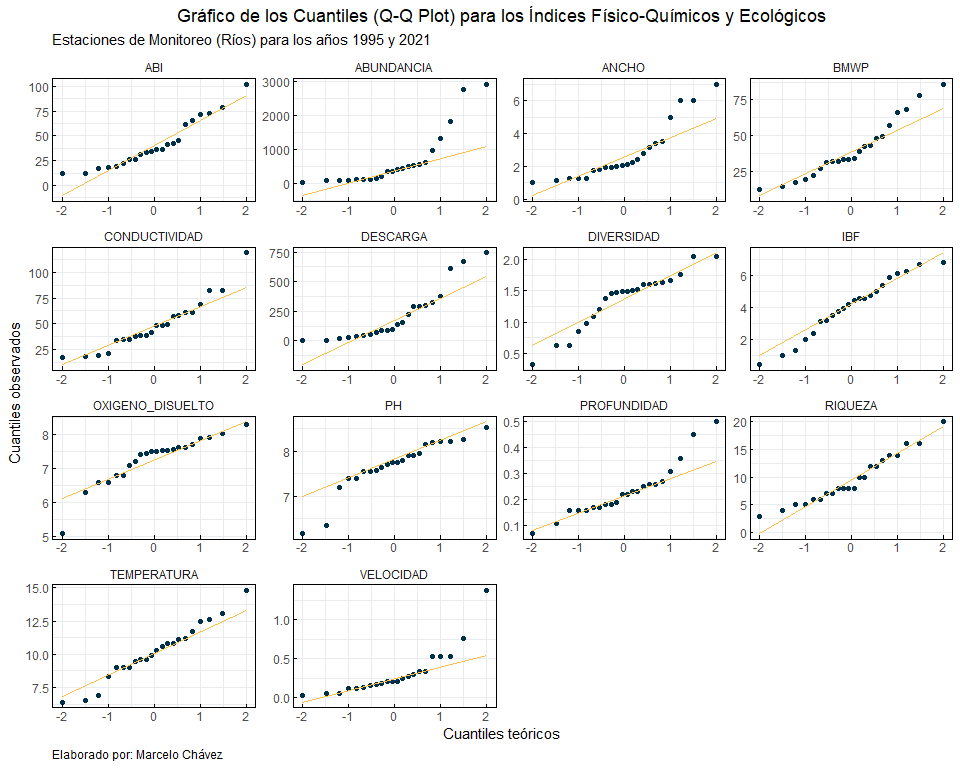
\includegraphics{CaracterizacionEcologica_files/figure-pdf/f_qqplot-1.png}

}

\end{figure}

\hypertarget{test-no-paramuxe9trico-de-shapiro-wilk-para-evaluar-la-normalidad-en-los-uxedndices-fuxedsico-quuxedmicos-y-ecoluxf3gicos}{%
\section{\texorpdfstring{Test No paramétrico de \textbf{Shapiro-Wilk}
para evaluar la normalidad en los Índices Físico-Químicos y
Ecológicos:}{Test No paramétrico de Shapiro-Wilk para evaluar la normalidad en los Índices Físico-Químicos y Ecológicos:}}\label{test-no-paramuxe9trico-de-shapiro-wilk-para-evaluar-la-normalidad-en-los-uxedndices-fuxedsico-quuxedmicos-y-ecoluxf3gicos}}

\begin{Shaded}
\begin{Highlighting}[numbers=left,,]
\CommentTok{\# Definir una función para aplicar el test de Shapiro{-}Wilk a todas las variables numéricas}
\NormalTok{shapiro\_test\_all }\OtherTok{\textless{}{-}} \ControlFlowTok{function}\NormalTok{(df) \{}
  
  \CommentTok{\# Filtrar solo las variables numéricas}
\NormalTok{  numeric\_vars }\OtherTok{\textless{}{-}}\NormalTok{ df[}\FunctionTok{sapply}\NormalTok{(df, is.numeric)]}
  
  \CommentTok{\# Crear una lista para almacenar los resultados del test}
\NormalTok{  test\_results }\OtherTok{\textless{}{-}} \FunctionTok{list}\NormalTok{()}
  
  \CommentTok{\# Iterar sobre cada variable numérica y aplicar el test de Shapiro{-}Wilk}
  \ControlFlowTok{for}\NormalTok{ (var\_name }\ControlFlowTok{in} \FunctionTok{names}\NormalTok{(numeric\_vars)) \{}
    
\NormalTok{    result }\OtherTok{\textless{}{-}} \FunctionTok{shapiro.test}\NormalTok{(numeric\_vars[[var\_name]])}
    
    \CommentTok{\# Redondear el estadístico W y el valor p a dos decimales}
\NormalTok{    result}\SpecialCharTok{$}\NormalTok{statistic }\OtherTok{\textless{}{-}} \FunctionTok{round}\NormalTok{(result}\SpecialCharTok{$}\NormalTok{statistic, }\DecValTok{2}\NormalTok{)}
    
\NormalTok{    result}\SpecialCharTok{$}\NormalTok{p.value }\OtherTok{\textless{}{-}} \FunctionTok{round}\NormalTok{(result}\SpecialCharTok{$}\NormalTok{p.value, }\DecValTok{2}\NormalTok{)}
    
\NormalTok{    test\_results[[var\_name]] }\OtherTok{\textless{}{-}}\NormalTok{ result}
\NormalTok{  \}}
  
  \CommentTok{\# Retornar los resultados como una lista}
  \FunctionTok{return}\NormalTok{(test\_results)}
\NormalTok{\}}

\CommentTok{\# Aplicar la función al dataframe indices\_fq\_ddc}
\NormalTok{shapiro\_results }\OtherTok{\textless{}{-}} \FunctionTok{shapiro\_test\_all}\NormalTok{(indices\_fq\_ddc)}

\CommentTok{\# Convertir los resultados en un tibble}
\NormalTok{results\_df }\OtherTok{\textless{}{-}}\NormalTok{ tibble}\SpecialCharTok{::}\FunctionTok{enframe}\NormalTok{(shapiro\_results,}
                              \AttributeTok{name =} \StringTok{"Variable"}\NormalTok{, }
                              \AttributeTok{value =} \StringTok{"Resultados"}\NormalTok{)}

\CommentTok{\# Extraer los estadísticos W y los valores p en columnas separadas}
\NormalTok{results\_df }\OtherTok{\textless{}{-}}\NormalTok{ results\_df }\SpecialCharTok{\%\textgreater{}\%}
  \FunctionTok{mutate}\NormalTok{(}\AttributeTok{W =} \FunctionTok{sapply}\NormalTok{(Resultados, }
                    \StringTok{"[["}\NormalTok{, }
                    \StringTok{"statistic"}\NormalTok{),}
         
         \AttributeTok{p\_value =} \FunctionTok{sapply}\NormalTok{(Resultados, }
                          \StringTok{"[["}\NormalTok{,}
                          \StringTok{"p.value"}\NormalTok{))}

\CommentTok{\# Seleccionar las columnas relevantes}
\NormalTok{results\_df }\OtherTok{\textless{}{-}}\NormalTok{ results\_df }\SpecialCharTok{\%\textgreater{}\%}
  \FunctionTok{select}\NormalTok{(Variable, W, p\_value)}

\CommentTok{\# Definir los niveles de significancia}
\NormalTok{significance\_levels }\OtherTok{\textless{}{-}} \FunctionTok{c}\NormalTok{(}\FloatTok{0.05}\NormalTok{, }\FloatTok{0.01}\NormalTok{, }\FloatTok{0.10}\NormalTok{)}

\CommentTok{\# Función para determinar si el valor p es mayor o menor que un nivel de significancia dado}
\NormalTok{check\_significance }\OtherTok{\textless{}{-}} \ControlFlowTok{function}\NormalTok{(p\_value, }
\NormalTok{                               significance\_level) \{}
  
  \ControlFlowTok{if}\NormalTok{ (p\_value }\SpecialCharTok{\textless{}}\NormalTok{ significance\_level) \{}
    \FunctionTok{return}\NormalTok{(}\StringTok{"Menor al $}\SpecialCharTok{\textbackslash{}\textbackslash{}}\StringTok{alpha$"}\NormalTok{)}
\NormalTok{  \} }\ControlFlowTok{else}\NormalTok{ \{}
    \FunctionTok{return}\NormalTok{(}\StringTok{"Mayor o igual $}\SpecialCharTok{\textbackslash{}\textbackslash{}}\StringTok{alpha$"}\NormalTok{)}
\NormalTok{  \}}
\NormalTok{\}}

\CommentTok{\# Aplicar la función a cada valor p y nivel de significancia}
\ControlFlowTok{for}\NormalTok{ (level }\ControlFlowTok{in}\NormalTok{ significance\_levels) \{}
  
\NormalTok{  results\_df }\OtherTok{\textless{}{-}}\NormalTok{ results\_df }\SpecialCharTok{\%\textgreater{}\%}
    \FunctionTok{mutate}\NormalTok{(}
      \SpecialCharTok{!!}\FunctionTok{paste0}\NormalTok{(}\StringTok{"Nivel de Significancia al "}\NormalTok{, }
\NormalTok{               level) }\SpecialCharTok{:}\ErrorTok{=} \FunctionTok{sapply}\NormalTok{(p\_value,}
\NormalTok{                                check\_significance, }
                                \AttributeTok{significance\_level =}\NormalTok{ level),}
      \SpecialCharTok{!!}\FunctionTok{paste0}\NormalTok{(}\StringTok{"Rechazas H0 al "}\NormalTok{,}
\NormalTok{               level) }\SpecialCharTok{:}\ErrorTok{=} \FunctionTok{ifelse}\NormalTok{(p\_value }\SpecialCharTok{\textless{}}\NormalTok{ level,}
                                \StringTok{"Sí"}\NormalTok{,}
                                \StringTok{"No"}\NormalTok{)}
\NormalTok{    )}
\NormalTok{\}}

\CommentTok{\# Mostrar la tabla actualizada}
\NormalTok{knitr}\SpecialCharTok{::}\FunctionTok{kable}\NormalTok{(results\_df, }\AttributeTok{format =} \StringTok{"markdown"}\NormalTok{)}
\end{Highlighting}
\end{Shaded}

\begin{longtable}[]{@{}
  >{\raggedright\arraybackslash}p{(\columnwidth - 16\tabcolsep) * \real{0.0939}}
  >{\raggedleft\arraybackslash}p{(\columnwidth - 16\tabcolsep) * \real{0.0276}}
  >{\raggedleft\arraybackslash}p{(\columnwidth - 16\tabcolsep) * \real{0.0442}}
  >{\raggedright\arraybackslash}p{(\columnwidth - 16\tabcolsep) * \real{0.1713}}
  >{\raggedright\arraybackslash}p{(\columnwidth - 16\tabcolsep) * \real{0.1105}}
  >{\raggedright\arraybackslash}p{(\columnwidth - 16\tabcolsep) * \real{0.1713}}
  >{\raggedright\arraybackslash}p{(\columnwidth - 16\tabcolsep) * \real{0.1105}}
  >{\raggedright\arraybackslash}p{(\columnwidth - 16\tabcolsep) * \real{0.1657}}
  >{\raggedright\arraybackslash}p{(\columnwidth - 16\tabcolsep) * \real{0.1050}}@{}}
\toprule\noalign{}
\begin{minipage}[b]{\linewidth}\raggedright
Variable
\end{minipage} & \begin{minipage}[b]{\linewidth}\raggedleft
W
\end{minipage} & \begin{minipage}[b]{\linewidth}\raggedleft
p\_value
\end{minipage} & \begin{minipage}[b]{\linewidth}\raggedright
Nivel de Significancia al 0.05
\end{minipage} & \begin{minipage}[b]{\linewidth}\raggedright
Rechazas H0 al 0.05
\end{minipage} & \begin{minipage}[b]{\linewidth}\raggedright
Nivel de Significancia al 0.01
\end{minipage} & \begin{minipage}[b]{\linewidth}\raggedright
Rechazas H0 al 0.01
\end{minipage} & \begin{minipage}[b]{\linewidth}\raggedright
Nivel de Significancia al 0.1
\end{minipage} & \begin{minipage}[b]{\linewidth}\raggedright
Rechazas H0 al 0.1
\end{minipage} \\
\midrule\noalign{}
\endhead
\bottomrule\noalign{}
\endlastfoot
ANCHO & 0.83 & 0.00 & Menor al \(\alpha\) & Sí & Menor al \(\alpha\) &
Sí & Menor al \(\alpha\) & Sí \\
PROFUNDIDAD & 0.90 & 0.03 & Menor al \(\alpha\) & Sí & Mayor o igual
\(\alpha\) & No & Menor al \(\alpha\) & Sí \\
VELOCIDAD & 0.75 & 0.00 & Menor al \(\alpha\) & Sí & Menor al \(\alpha\)
& Sí & Menor al \(\alpha\) & Sí \\
DESCARGA & 0.83 & 0.00 & Menor al \(\alpha\) & Sí & Menor al \(\alpha\)
& Sí & Menor al \(\alpha\) & Sí \\
PH & 0.88 & 0.01 & Menor al \(\alpha\) & Sí & Mayor o igual \(\alpha\) &
No & Menor al \(\alpha\) & Sí \\
TEMPERATURA & 0.98 & 0.84 & Mayor o igual \(\alpha\) & No & Mayor o
igual \(\alpha\) & No & Mayor o igual \(\alpha\) & No \\
OXIGENO\_DISUELTO & 0.88 & 0.01 & Menor al \(\alpha\) & Sí & Mayor o
igual \(\alpha\) & No & Menor al \(\alpha\) & Sí \\
CONDUCTIVIDAD & 0.92 & 0.07 & Mayor o igual \(\alpha\) & No & Mayor o
igual \(\alpha\) & No & Menor al \(\alpha\) & Sí \\
RIQUEZA & 0.95 & 0.33 & Mayor o igual \(\alpha\) & No & Mayor o igual
\(\alpha\) & No & Mayor o igual \(\alpha\) & No \\
ABUNDANCIA & 0.71 & 0.00 & Menor al \(\alpha\) & Sí & Menor al
\(\alpha\) & Sí & Menor al \(\alpha\) & Sí \\
DIVERSIDAD & 0.79 & 0.00 & Menor al \(\alpha\) & Sí & Menor al
\(\alpha\) & Sí & Menor al \(\alpha\) & Sí \\
ABI & 0.91 & 0.04 & Menor al \(\alpha\) & Sí & Mayor o igual \(\alpha\)
& No & Menor al \(\alpha\) & Sí \\
BMWP & 0.94 & 0.16 & Mayor o igual \(\alpha\) & No & Mayor o igual
\(\alpha\) & No & Mayor o igual \(\alpha\) & No \\
IBF & 0.96 & 0.60 & Mayor o igual \(\alpha\) & No & Mayor o igual
\(\alpha\) & No & Mayor o igual \(\alpha\) & No \\
\end{longtable}

\hypertarget{comprobaciuxf3n-de-hipuxf3tesis-para-anuxe1lisis-normalidad}{%
\section{Comprobación de hipótesis para análisis
normalidad:}\label{comprobaciuxf3n-de-hipuxf3tesis-para-anuxe1lisis-normalidad}}

Para la comprobaciónd de normalidad se ha planteado la siguiente prueba
de hipótesis:

\(H_{0}:\) Las variables provienen de una Distribución Normal

\(H_{1}:\) Las variables NO provienen de una Distribución Normal

\begin{quote}
\textbf{Análisis:} De igual forma en un contexto general los indicadores
físico-químicos y ecológicos, con un nivel de significancia del 5\%. De
las 14 variables, 5 presentan normalidad y el resto de variables no lo
son. Este resultado nos conduce a generalizar que para todo el conjunto
de datos es necesario reducir la dimensionalidad y/o aplicar un
\textbf{método No Paramétrico} para descubrir clústers o taxonomías
entre las unidades de estudio.
\end{quote}

\hypertarget{anuxe1lisis-factorial-por-componentes-principales}{%
\chapter{Análisis Factorial por Componentes
Principales:}\label{anuxe1lisis-factorial-por-componentes-principales}}

El \textbf{análisis factorial} en un contexto de rigurosidad estadística
presente los siguientes pasos:

\begin{itemize}
\item
  Matriz de correlaciones y su significancia estadística
\item
  Determinante de la matriz de correlaciones
\item
  Prueba de esfericidad de Bartlett
\item
  Comprobación de hipótesis para el análisis factorial por componentes
  principales
\item
  Gráfico de Sedimentación
\item
  Proporción de Varianza Acumulada
\item
  Componentes Principales
\item
  Autovalores y Varianzas
\item
  Círculo de las Correlaciones
\item
  Variables versus Dimensiones
\item
  Biplot (variables versus las estaciones de monitoreo)
\item
  Índice Multivariante
\end{itemize}

\hypertarget{matriz-de-correlaciones}{%
\section{Matriz de Correlaciones:}\label{matriz-de-correlaciones}}

\begin{Shaded}
\begin{Highlighting}[numbers=left,,]
\CommentTok{\# Calcular correlaciones y p{-}values}
\NormalTok{correlation\_matrix }\OtherTok{\textless{}{-}} \FunctionTok{cor}\NormalTok{(indices\_fq\_ddc)}
\NormalTok{p\_values }\OtherTok{\textless{}{-}} \FunctionTok{cor.mtest}\NormalTok{(indices\_fq\_ddc)}\SpecialCharTok{$}\NormalTok{p}

\CommentTok{\# Convertir p{-}values en asteriscos de acuerdo con el nivel de significancia}
\NormalTok{significant\_level }\OtherTok{\textless{}{-}} \FunctionTok{ifelse}\NormalTok{(p\_values }\SpecialCharTok{\textless{}} \FloatTok{0.001}\NormalTok{, }\StringTok{"***"}\NormalTok{,}
                            \FunctionTok{ifelse}\NormalTok{(p\_values }\SpecialCharTok{\textless{}} \FloatTok{0.01}\NormalTok{, }\StringTok{"**"}\NormalTok{,}
                                   \FunctionTok{ifelse}\NormalTok{(p\_values }\SpecialCharTok{\textless{}} \FloatTok{0.05}\NormalTok{, }\StringTok{"*"}\NormalTok{, }\StringTok{""}\NormalTok{)))}

\CommentTok{\# Crear gráfico}
\FunctionTok{ggplot}\NormalTok{(}\AttributeTok{data =} \FunctionTok{melt}\NormalTok{(}\FunctionTok{round}\NormalTok{(correlation\_matrix, }\DecValTok{2}\NormalTok{)), }\FunctionTok{aes}\NormalTok{(}\AttributeTok{x =}\NormalTok{ Var1, }\AttributeTok{y =}\NormalTok{ Var2, }\AttributeTok{fill =}\NormalTok{ value)) }\SpecialCharTok{+}
    \FunctionTok{geom\_tile}\NormalTok{() }\SpecialCharTok{+}
    \FunctionTok{geom\_text}\NormalTok{(}\FunctionTok{aes}\NormalTok{(}\AttributeTok{label =} \FunctionTok{paste}\NormalTok{(}\FunctionTok{round}\NormalTok{(value, }\DecValTok{2}\NormalTok{), significant\_level)), }\AttributeTok{color =} \StringTok{"black"}\NormalTok{, }\AttributeTok{size =} \DecValTok{4}\NormalTok{) }\SpecialCharTok{+}
    \FunctionTok{labs}\NormalTok{(}
        \AttributeTok{title =} \StringTok{"Mapa de calor de correlaciones"}\NormalTok{,}
        \AttributeTok{x =} \StringTok{""}\NormalTok{,}
        \AttributeTok{y =} \StringTok{""}\NormalTok{,}
        \AttributeTok{fill =} \StringTok{"Nivel de Correlación"}\NormalTok{,}
        \AttributeTok{caption =} \StringTok{"Elaborado por: Karina Hernández"}
\NormalTok{    ) }\SpecialCharTok{+}
    \FunctionTok{scale\_fill\_gradient}\NormalTok{(}\AttributeTok{low =} \StringTok{"\#caf0f8"}\NormalTok{, }\AttributeTok{high =} \StringTok{"\#2a9d8f"}\NormalTok{) }\SpecialCharTok{+}
    \FunctionTok{theme\_minimal}\NormalTok{() }\SpecialCharTok{+}
    \FunctionTok{theme}\NormalTok{(}
        \AttributeTok{axis.text.x =} \FunctionTok{element\_text}\NormalTok{(}\AttributeTok{angle =} \DecValTok{90}\NormalTok{, }\AttributeTok{vjust =} \FloatTok{0.5}\NormalTok{, }\AttributeTok{hjust =} \DecValTok{1}\NormalTok{),}
        \AttributeTok{axis.title.x =} \FunctionTok{element\_text}\NormalTok{(}\AttributeTok{angle =} \DecValTok{90}\NormalTok{),}
        \AttributeTok{axis.title.y =} \FunctionTok{element\_text}\NormalTok{(}\AttributeTok{angle =} \DecValTok{0}\NormalTok{),}
        \AttributeTok{panel.grid =} \FunctionTok{element\_line}\NormalTok{(}\AttributeTok{color =} \StringTok{"\#e9ecef"}\NormalTok{, }\AttributeTok{linewidth =} \FloatTok{0.5}\NormalTok{),  }\CommentTok{\# Cambio a linewidth}
        \AttributeTok{panel.border =} \FunctionTok{element\_rect}\NormalTok{(}\AttributeTok{color =} \StringTok{"black"}\NormalTok{, }\AttributeTok{fill =} \ConstantTok{NA}\NormalTok{),}
        \AttributeTok{axis.ticks =} \FunctionTok{element\_line}\NormalTok{(}\AttributeTok{color =} \StringTok{"black"}\NormalTok{),}
        \AttributeTok{axis.line =} \FunctionTok{element\_blank}\NormalTok{(),}
        \AttributeTok{plot.title =} \FunctionTok{element\_text}\NormalTok{(}\AttributeTok{hjust =} \FloatTok{0.5}\NormalTok{),}
        \AttributeTok{plot.caption =} \FunctionTok{element\_text}\NormalTok{(}\AttributeTok{hjust =} \DecValTok{0}\NormalTok{),}
        \AttributeTok{axis.ticks.length =} \FunctionTok{unit}\NormalTok{(}\SpecialCharTok{{-}}\FloatTok{0.1}\NormalTok{, }\StringTok{"cm"}\NormalTok{)}
\NormalTok{    )}
\end{Highlighting}
\end{Shaded}

\begin{figure}[tb]

{\centering 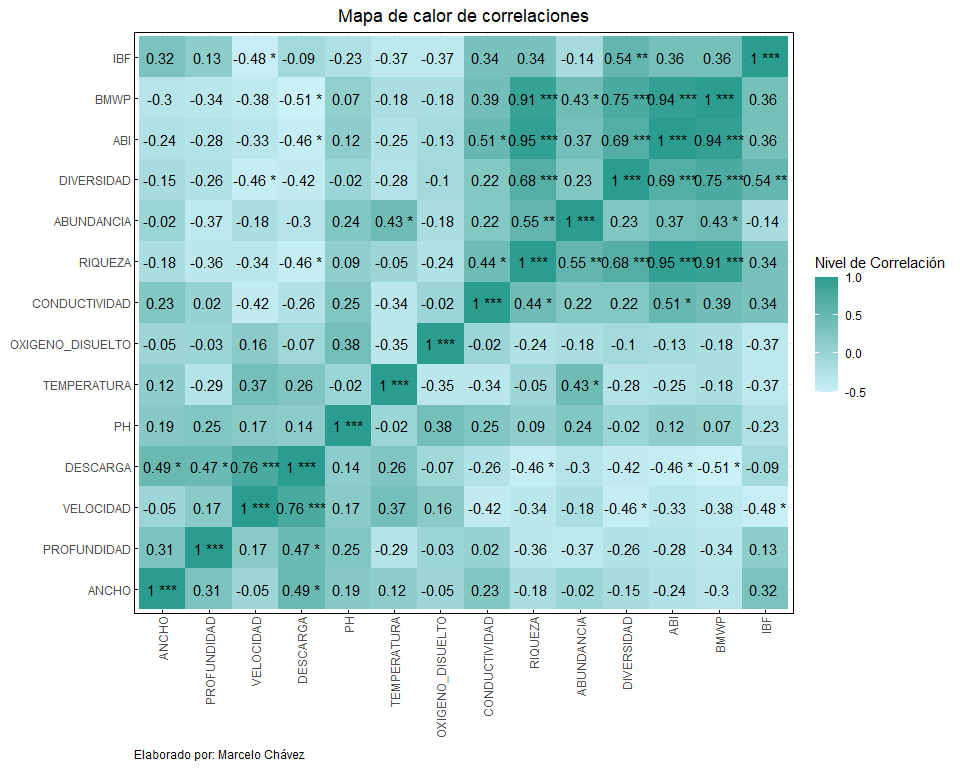
\includegraphics{CaracterizacionEcologica_files/figure-pdf/correlaciones-1.png}

}

\end{figure}

\begin{quote}
Es importante conocer que el nivel de significancia de la matriz de
correlaciones para definir variables que a más de tener un buen nivel de
correlación, es significativo estadísticamente.
\end{quote}

\begin{quote}
\(\\p-value < 0.001 (***):\) Es significativa la correlación al 99\%
\(\\p-value < 0.05 (**):\) Es significativa la correlación al 95\%
\(\\p-value < 0.01 (*):\) Es significativa la correlación al 90\%
\end{quote}

\hypertarget{determinante-de-la-matriz-de-correlaciones}{%
\section{Determinante de la matriz de
correlaciones}\label{determinante-de-la-matriz-de-correlaciones}}

\begin{Shaded}
\begin{Highlighting}[numbers=left,,]
\FunctionTok{det}\NormalTok{(}\FunctionTok{cor}\NormalTok{(indices\_fq\_ddc))}
\end{Highlighting}
\end{Shaded}

\begin{verbatim}
[1] 2.706342e-07
\end{verbatim}

\begin{quote}
Si están correlacionadas, el determinantes de la matriz de correlaciones
será próximo a cero. De lo contrario el \textbf{Análisis Factorial} no
es viable.
\end{quote}

\hypertarget{prueba-de-esfericidad-de-bartlett}{%
\section{Prueba de esfericidad de
Bartlett:}\label{prueba-de-esfericidad-de-bartlett}}

\begin{Shaded}
\begin{Highlighting}[numbers=left,,]
\FunctionTok{KMO}\NormalTok{(indices\_fq\_ddc)}
\end{Highlighting}
\end{Shaded}

\begin{verbatim}
Kaiser-Meyer-Olkin factor adequacy
Call: KMO(r = indices_fq_ddc)
Overall MSA =  0.44
MSA for each item = 
           ANCHO      PROFUNDIDAD        VELOCIDAD         DESCARGA 
            0.26             0.65             0.35             0.41 
              PH      TEMPERATURA OXIGENO_DISUELTO    CONDUCTIVIDAD 
            0.36             0.26             0.17             0.61 
         RIQUEZA       ABUNDANCIA       DIVERSIDAD              ABI 
            0.60             0.42             0.61             0.48 
            BMWP              IBF 
            0.58             0.55 
\end{verbatim}

\begin{Shaded}
\begin{Highlighting}[numbers=left,,]
\FunctionTok{cortest.bartlett}\NormalTok{(}\FunctionTok{cor}\NormalTok{(indices\_fq\_ddc))}
\end{Highlighting}
\end{Shaded}

\begin{verbatim}
$chisq
[1] 1413.954

$p.value
[1] 3.472263e-236

$df
[1] 91
\end{verbatim}

\begin{quote}
Un KMO de 0.44 es considerado bajo y podría sugerir que un análisis
factorial puede no ser adecuado para estos datos. Sin embargo, la prueba
de Bartlett tiene un p-valor menor al nivel de significancia del 5\%, lo
que indica que las variables están correlacionadas y que, por lo tanto,
podría justificarse aplicar un método multivariante para reducción de
dimensionalidad.
\end{quote}

\begin{quote}
La hipótesis nula es que la matriz de correlaciones es una matriz
identidad, lo que significa que no existirían correlaciones
significativas, por lo que el modelo factorial no sería pertinente.
\end{quote}

\hypertarget{comprobaciuxf3n-de-hipuxf3tesis-para-el-anuxe1lisis-factorial-por-componentes-principales}{%
\section{Comprobación de hipótesis para el análisis factorial por
componentes
principales}\label{comprobaciuxf3n-de-hipuxf3tesis-para-el-anuxe1lisis-factorial-por-componentes-principales}}

\(H_{0}:\) Existe esfericidad

\(H_{1}:\) No existe esfericidad

\begin{quote}
La esfericidad implica que todas las variables tienen la misma varianza
y que no hay correlaciones entre ellas.
\end{quote}

\begin{quote}
De aquí que el valor del \emph{KMO} de 0.44 y su p-valor es menor al
95\% de confianza. Por lo tanto: Rechazamos \(H_{0}\), y concluimos que
es factible estadísticamente realizar la reducción de dimensiones a
través de un \textbf{Análisis Factorial por Componentes Principales}
\end{quote}

\hypertarget{gruxe1fico-de-sedimentaciuxf3n}{%
\section{Gráfico de
Sedimentación:}\label{gruxe1fico-de-sedimentaciuxf3n}}

\begin{Shaded}
\begin{Highlighting}[numbers=left,,]
\FunctionTok{scree}\NormalTok{(indices\_fq\_ddc,}
      \AttributeTok{main =}\StringTok{"Gráfico de Sedimentación"}\NormalTok{)}
\end{Highlighting}
\end{Shaded}

\begin{figure}[tb]

{\centering 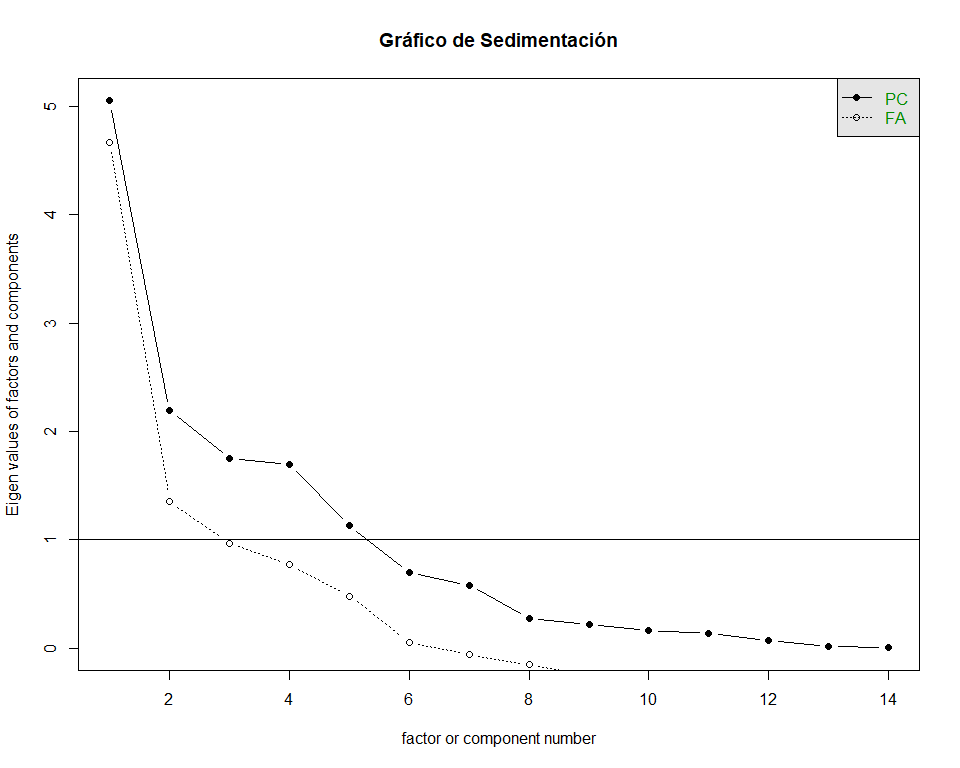
\includegraphics{CaracterizacionEcologica_files/figure-pdf/sedimentacion-1.png}

}

\end{figure}

\hypertarget{proporciuxf3n-de-varianza-acumulada}{%
\section{Proporción de varianza
acumulada:}\label{proporciuxf3n-de-varianza-acumulada}}

\begin{Shaded}
\begin{Highlighting}[numbers=left,,]
\CommentTok{\# Cálculo de los autovalores y autovectores:}
\NormalTok{value\_pro}\OtherTok{\textless{}{-}}\FunctionTok{eigen}\NormalTok{(}\FunctionTok{cor}\NormalTok{(indices\_fq\_ddc))}

\NormalTok{Acumulado }\OtherTok{\textless{}{-}} \FunctionTok{cumsum}\NormalTok{(value\_pro}\SpecialCharTok{$}\NormalTok{values)}

\NormalTok{Prop.acumulado }\OtherTok{\textless{}{-}}\NormalTok{ Acumulado}\SpecialCharTok{/}\FunctionTok{sum}\NormalTok{(value\_pro}\SpecialCharTok{$}\NormalTok{values)}

\NormalTok{val.prop.porce }\OtherTok{\textless{}{-}} \FunctionTok{data.frame}\NormalTok{(value\_pro}\SpecialCharTok{$}\NormalTok{values,}
\NormalTok{                             Acumulado,}
\NormalTok{                             Prop.acumulado)}

\FunctionTok{row.names}\NormalTok{(val.prop.porce) }\OtherTok{=} \FunctionTok{c}\NormalTok{(}\FunctionTok{expression}\NormalTok{(lambda[}\DecValTok{1}\NormalTok{]),}
                              \FunctionTok{expression}\NormalTok{(lambda[}\DecValTok{2}\NormalTok{]),}
                              \FunctionTok{expression}\NormalTok{(lambda[}\DecValTok{3}\NormalTok{]),}
                              \FunctionTok{expression}\NormalTok{(lambda[}\DecValTok{4}\NormalTok{]),}
                              \FunctionTok{expression}\NormalTok{(lambda[}\DecValTok{5}\NormalTok{]),}
                              \FunctionTok{expression}\NormalTok{(lambda[}\DecValTok{6}\NormalTok{]),}
                              \FunctionTok{expression}\NormalTok{(lambda[}\DecValTok{7}\NormalTok{]),}
                              \FunctionTok{expression}\NormalTok{(lambda[}\DecValTok{8}\NormalTok{]),}
                              \FunctionTok{expression}\NormalTok{(lambda[}\DecValTok{9}\NormalTok{]),}
                              \FunctionTok{expression}\NormalTok{(lambda[}\DecValTok{10}\NormalTok{]),}
                              \FunctionTok{expression}\NormalTok{(lambda[}\DecValTok{11}\NormalTok{]),}
                              \FunctionTok{expression}\NormalTok{(lambda[}\DecValTok{12}\NormalTok{]),}
                              \FunctionTok{expression}\NormalTok{(lambda[}\DecValTok{13}\NormalTok{]),}
                              \FunctionTok{expression}\NormalTok{(lambda[}\DecValTok{14}\NormalTok{]))}
                              
\FunctionTok{colnames}\NormalTok{(val.prop.porce) }\OtherTok{\textless{}{-}} \FunctionTok{c}\NormalTok{(}\StringTok{"Valor Propio"}\NormalTok{,}
                              \StringTok{"Acumulado"}\NormalTok{,}
                              \StringTok{"Prop. Acumulado"}\NormalTok{)}
\FunctionTok{kable}\NormalTok{(val.prop.porce,}
      \AttributeTok{caption =} \StringTok{"Valores propios desde la matriz de correlaciones"}\NormalTok{,}
      \AttributeTok{digits =} \DecValTok{2}\NormalTok{,}
      \AttributeTok{format.args =} \FunctionTok{list}\NormalTok{(}\AttributeTok{decimal.mark =}\StringTok{","}\NormalTok{)) }\SpecialCharTok{\%\textgreater{}\%}
  \FunctionTok{row\_spec}\NormalTok{(}\AttributeTok{row =} \DecValTok{5}\NormalTok{,}
           \AttributeTok{background=}\StringTok{"\#a7c957"}\NormalTok{,}
           \AttributeTok{bold=}\NormalTok{T)}
\end{Highlighting}
\end{Shaded}

\begin{longtable}[t]{lrrr}
\caption{Valores propios desde la matriz de correlaciones}\\
\toprule
 & Valor Propio & Acumulado & Prop. Acumulado\\
\midrule
lambda[1] & 4,72 & 4,72 & 0,34\\
lambda[2] & 2,27 & 6,99 & 0,50\\
lambda[3] & 1,82 & 8,82 & 0,63\\
lambda[4] & 1,70 & 10,51 & 0,75\\
\cellcolor[HTML]{a7c957}{\textbf{lambda[5]}} & \cellcolor[HTML]{a7c957}{\textbf{1,11}} & \cellcolor[HTML]{a7c957}{\textbf{11,62}} & \cellcolor[HTML]{a7c957}{\textbf{0,83}}\\
\addlinespace
lambda[6] & 0,90 & 12,52 & 0,89\\
lambda[7] & 0,52 & 13,05 & 0,93\\
lambda[8] & 0,31 & 13,36 & 0,95\\
lambda[9] & 0,26 & 13,62 & 0,97\\
lambda[10] & 0,18 & 13,80 & 0,99\\
\addlinespace
lambda[11] & 0,10 & 13,90 & 0,99\\
lambda[12] & 0,08 & 13,97 & 1,00\\
lambda[13] & 0,02 & 13,99 & 1,00\\
lambda[14] & 0,01 & 14,00 & 1,00\\
\bottomrule
\end{longtable}

\begin{quote}
El \textbf{Valor Propio} de la matriz de correlaciones cuando desciende
hasta 1 sugiere que el número de componentes o factores que pueden
explicar la variabilidad de todo el conjunto de datos está en un
\(\lambda=5\) y lo corrobora el \textbf{Gráfico de Sedimentación}
\end{quote}

\hypertarget{componentes-principales}{%
\section{Componentes Principales:}\label{componentes-principales}}

\begin{Shaded}
\begin{Highlighting}[numbers=left,,]
\NormalTok{pca }\OtherTok{\textless{}{-}} \FunctionTok{prcomp}\NormalTok{(indices\_fq\_ddc,}
              \AttributeTok{scale=}\ConstantTok{TRUE}\NormalTok{,}
              \AttributeTok{center =} \ConstantTok{TRUE}\NormalTok{,}
              \AttributeTok{method =} \StringTok{"varimax"}\NormalTok{)}
\FunctionTok{summary}\NormalTok{(pca)}
\end{Highlighting}
\end{Shaded}

\begin{verbatim}
Importance of components:
                         PC1    PC2    PC3    PC4     PC5     PC6     PC7
Standard deviation     2.172 1.5080 1.3503 1.3036 1.05141 0.95050 0.72437
Proportion of Variance 0.337 0.1624 0.1302 0.1214 0.07896 0.06453 0.03748
Cumulative Proportion  0.337 0.4994 0.6297 0.7511 0.83002 0.89456 0.93204
                           PC8     PC9   PC10   PC11    PC12    PC13    PC14
Standard deviation     0.55491 0.51189 0.4216 0.3153 0.27573 0.14732 0.08124
Proportion of Variance 0.02199 0.01872 0.0127 0.0071 0.00543 0.00155 0.00047
Cumulative Proportion  0.95403 0.97275 0.9855 0.9926 0.99798 0.99953 1.00000
\end{verbatim}

\hypertarget{autovalores-y-varianzas}{%
\section{Autovalores y varianzas:}\label{autovalores-y-varianzas}}

\begin{Shaded}
\begin{Highlighting}[numbers=left,,]
\FunctionTok{get\_eig}\NormalTok{(pca)}
\end{Highlighting}
\end{Shaded}

\begin{verbatim}
        eigenvalue variance.percent cumulative.variance.percent
Dim.1  4.717836203      33.69883002                    33.69883
Dim.2  2.274213490      16.24438207                    49.94321
Dim.3  1.823386036      13.02418597                    62.96740
Dim.4  1.699435601      12.13882572                    75.10622
Dim.5  1.105467492       7.89619637                    83.00242
Dim.6  0.903448292       6.45320209                    89.45562
Dim.7  0.524706456       3.74790326                    93.20353
Dim.8  0.307925627       2.19946876                    95.40299
Dim.9  0.262032510       1.87166079                    97.27466
Dim.10 0.177786579       1.26990413                    98.54456
Dim.11 0.099431722       0.71022659                    99.25479
Dim.12 0.076026874       0.54304910                    99.79783
Dim.13 0.021703083       0.15502202                    99.95286
Dim.14 0.006600033       0.04714309                   100.00000
\end{verbatim}

\begin{quote}
Al analizar los componentes principales podemos observar que en el
\textbf{Componente 5} se explica el \textbf{83\%} de la varianza de
todas las dimensiones
\end{quote}

\hypertarget{cuxedrculo-de-correlaciones}{%
\section{Círculo de correlaciones:}\label{cuxedrculo-de-correlaciones}}

\begin{Shaded}
\begin{Highlighting}[numbers=left,,]
\FunctionTok{fviz\_pca\_var}\NormalTok{(pca,}
             \AttributeTok{col.var=}\StringTok{"steelblue"}\NormalTok{) }\SpecialCharTok{+} 
  \FunctionTok{theme\_minimal}\NormalTok{()}
\end{Highlighting}
\end{Shaded}

\begin{figure}[tb]

{\centering 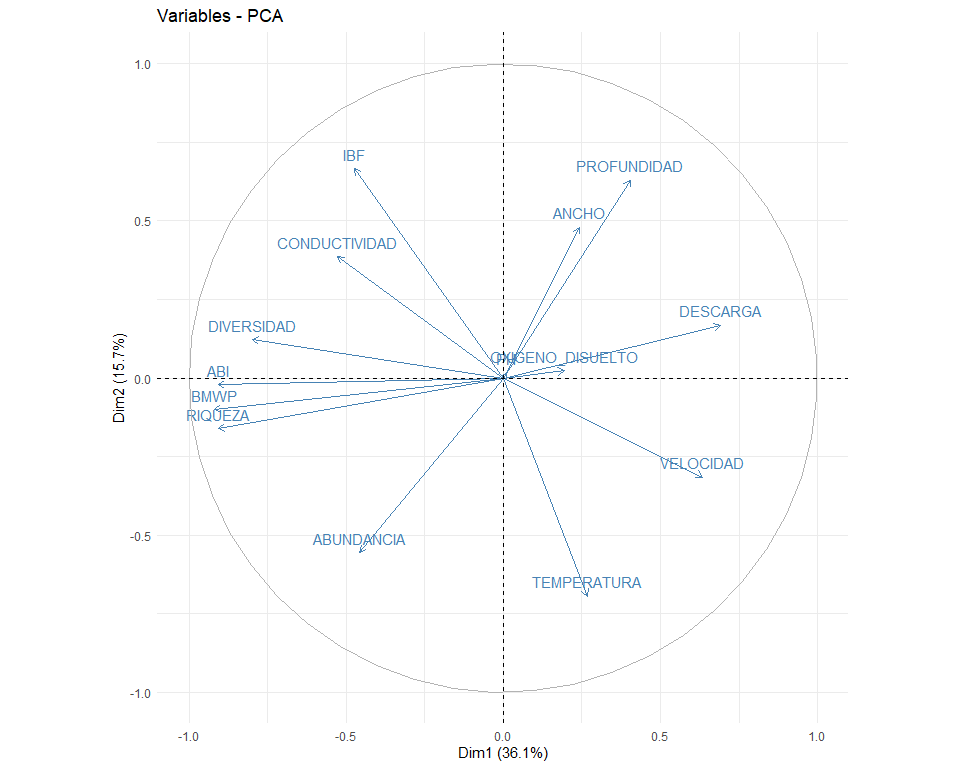
\includegraphics{CaracterizacionEcologica_files/figure-pdf/circulo_correlaciones-1.png}

}

\end{figure}

\begin{quote}
En el círculo de las correlaciones es una representación gráfica de las
correlaciones entre las variables originales y los componentes
principales extraídos durante el análisis factorial. Cada variable
original se representa como un vector en el espacio de los componentes
principales, donde la longitud del vector indica la correlación entre
esa variable y el componente principal correspondiente, y la dirección
del vector indica la dirección en la que esa variable contribuye al
componente principal. Por ejemplo, al examinar el círculo de
correlaciones, podemos observar que las variables \textbf{ABI, BMWP y
RIQUEZA} están inversamente correlacionadas con la Dimensión 2. Por otro
lado, las variables \textbf{ANCHO y PROFUNDIDAD} muestran una
correlación más fuerte con la Dimensión 1. En resumen, el círculo de
correlaciones proporciona una representación visual que ayuda a entender
cómo las variables originales están relacionadas y contribuyen a la
estructura de los componentes principales identificados durante el
análisis factorial
\end{quote}

\begin{Shaded}
\begin{Highlighting}[numbers=left,,]
\FunctionTok{fviz\_screeplot}\NormalTok{(pca,}
               \AttributeTok{ncp =} \DecValTok{5}\NormalTok{,}
               \AttributeTok{barfill =} \StringTok{"\#3fc1c0"}\NormalTok{,}
               \AttributeTok{barcolor =} \StringTok{"\#3fc1c0"}\NormalTok{,}
               \AttributeTok{addlabels =} \ConstantTok{TRUE}\NormalTok{,}
               \AttributeTok{ylab =} \StringTok{"Porcentaje de varianza explicada"}\NormalTok{,}
               \AttributeTok{xlab =} \StringTok{"Dimensiones"}\NormalTok{,}
               \AttributeTok{main =} \StringTok{"Porcentaje de varianza explicada por componente (Scree plot)"}\NormalTok{,}
               \AttributeTok{hjust =} \SpecialCharTok{{-}}\FloatTok{0.3}\NormalTok{) }\SpecialCharTok{+}
  \FunctionTok{theme}\NormalTok{(}\AttributeTok{plot.title =} \FunctionTok{element\_text}\NormalTok{(}\AttributeTok{size =} \DecValTok{14}\NormalTok{, }\AttributeTok{face =} \StringTok{"bold"}\NormalTok{),}
        \AttributeTok{plot.caption =} \FunctionTok{element\_text}\NormalTok{(}\AttributeTok{size =} \DecValTok{8}\NormalTok{, }\AttributeTok{face =} \StringTok{"italic"}\NormalTok{)) }\SpecialCharTok{+}
  \FunctionTok{labs}\NormalTok{(}\AttributeTok{caption =} \StringTok{"Elaborado por: Karina Hernández"}\NormalTok{) }\SpecialCharTok{+}
  \FunctionTok{theme\_minimal}\NormalTok{() }\SpecialCharTok{+}
    \FunctionTok{theme}\NormalTok{(}
        \AttributeTok{axis.text.x =} \FunctionTok{element\_text}\NormalTok{(}\AttributeTok{angle =} \DecValTok{90}\NormalTok{, }\AttributeTok{vjust =} \FloatTok{0.5}\NormalTok{, }\AttributeTok{hjust =} \DecValTok{1}\NormalTok{),}
        \AttributeTok{axis.title.x =} \FunctionTok{element\_text}\NormalTok{(}\AttributeTok{angle =} \DecValTok{90}\NormalTok{),}
        \AttributeTok{axis.title.y =} \FunctionTok{element\_text}\NormalTok{(}\AttributeTok{angle =} \DecValTok{0}\NormalTok{),}
        \AttributeTok{panel.grid =} \FunctionTok{element\_line}\NormalTok{(}\AttributeTok{color =} \StringTok{"\#e9ecef"}\NormalTok{, }\AttributeTok{linewidth =} \FloatTok{0.5}\NormalTok{),  }\CommentTok{\# Cambio a linewidth}
        \AttributeTok{panel.border =} \FunctionTok{element\_rect}\NormalTok{(}\AttributeTok{color =} \StringTok{"black"}\NormalTok{, }\AttributeTok{fill =} \ConstantTok{NA}\NormalTok{),}
        \AttributeTok{axis.ticks =} \FunctionTok{element\_line}\NormalTok{(}\AttributeTok{color =} \StringTok{"black"}\NormalTok{),}
        \AttributeTok{axis.line =} \FunctionTok{element\_blank}\NormalTok{(),}
        \AttributeTok{plot.title =} \FunctionTok{element\_text}\NormalTok{(}\AttributeTok{hjust =} \FloatTok{0.5}\NormalTok{),}
        \AttributeTok{plot.caption =} \FunctionTok{element\_text}\NormalTok{(}\AttributeTok{hjust =} \DecValTok{0}\NormalTok{),}
        \AttributeTok{axis.ticks.length =} \FunctionTok{unit}\NormalTok{(}\SpecialCharTok{{-}}\FloatTok{0.1}\NormalTok{, }\StringTok{"cm"}\NormalTok{)}
\NormalTok{    )}
\end{Highlighting}
\end{Shaded}

\begin{figure}[tb]

{\centering 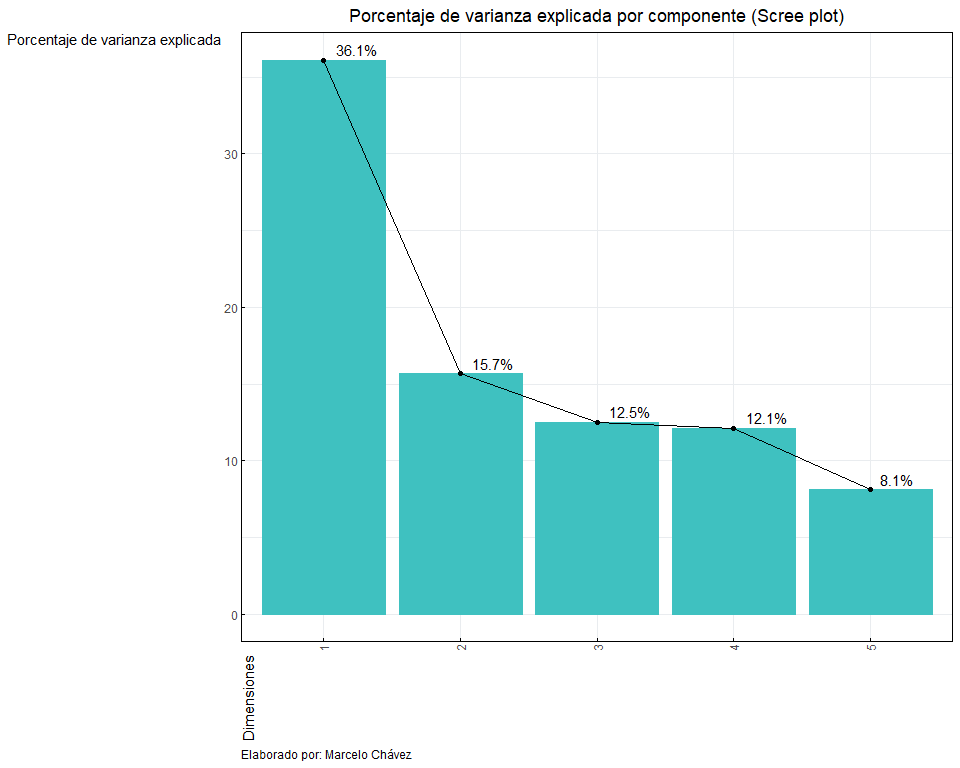
\includegraphics{CaracterizacionEcologica_files/figure-pdf/screeplot-1.png}

}

\end{figure}

\hypertarget{variables-versus-dimensiones}{%
\section{Variables versus
Dimensiones:}\label{variables-versus-dimensiones}}

\begin{Shaded}
\begin{Highlighting}[numbers=left,,]
\FunctionTok{fviz\_pca\_var}\NormalTok{(pca,}
             \AttributeTok{col.var=}\StringTok{"contrib"}\NormalTok{,}
             \AttributeTok{gradient.cols =} \FunctionTok{c}\NormalTok{(}\StringTok{"\#00AFBB"}\NormalTok{, }\StringTok{"\#E7B800"}\NormalTok{, }\StringTok{"\#FC4E07"}\NormalTok{),}
             \AttributeTok{repel =} \ConstantTok{TRUE}\NormalTok{)}
\end{Highlighting}
\end{Shaded}

\begin{figure}[tb]

{\centering 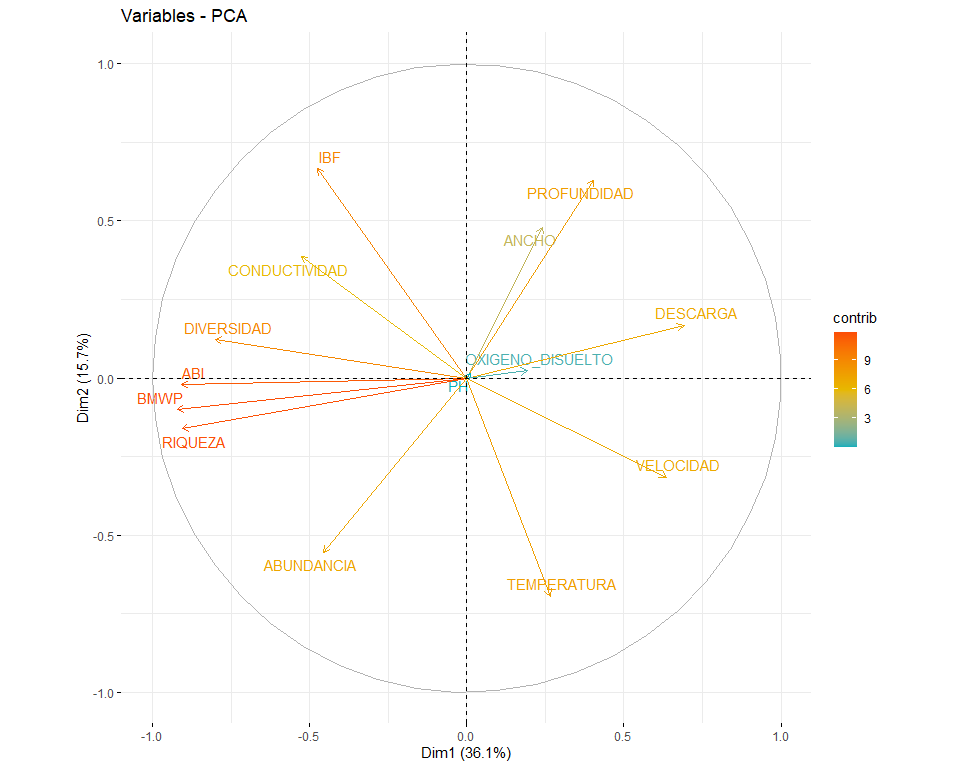
\includegraphics{CaracterizacionEcologica_files/figure-pdf/variables_dimensiones-1.png}

}

\end{figure}

\begin{quote}
Es fundamental examinar el nivel de contribución de las variables a cada
uno de los componentes principales. En este sentido, observamos que
variables como \textbf{ABI, BMWP y RIQUEZA} destacan por su
significativa contribución a la \textbf{Dimensión 2}. Sin embargo, al
considerar \textbf{OXÍGENO y PH}, a pesar de ubicarse en los mismos
componentes, la longitud de sus vectores indica una contribución mínima
al modelo factorial en construcción.
\end{quote}

\hypertarget{biplot-variables-versus-las-estaciones-de-monitoreo}{%
\section{Biplot (variables versus las estaciones de
monitoreo)}\label{biplot-variables-versus-las-estaciones-de-monitoreo}}

\begin{Shaded}
\begin{Highlighting}[numbers=left,,]
\CommentTok{\# Biplot of individuals and variables}
\FunctionTok{fviz\_pca\_biplot}\NormalTok{(pca, }\AttributeTok{repel =} \ConstantTok{TRUE}\NormalTok{)}
\end{Highlighting}
\end{Shaded}

\begin{figure}[tb]

{\centering 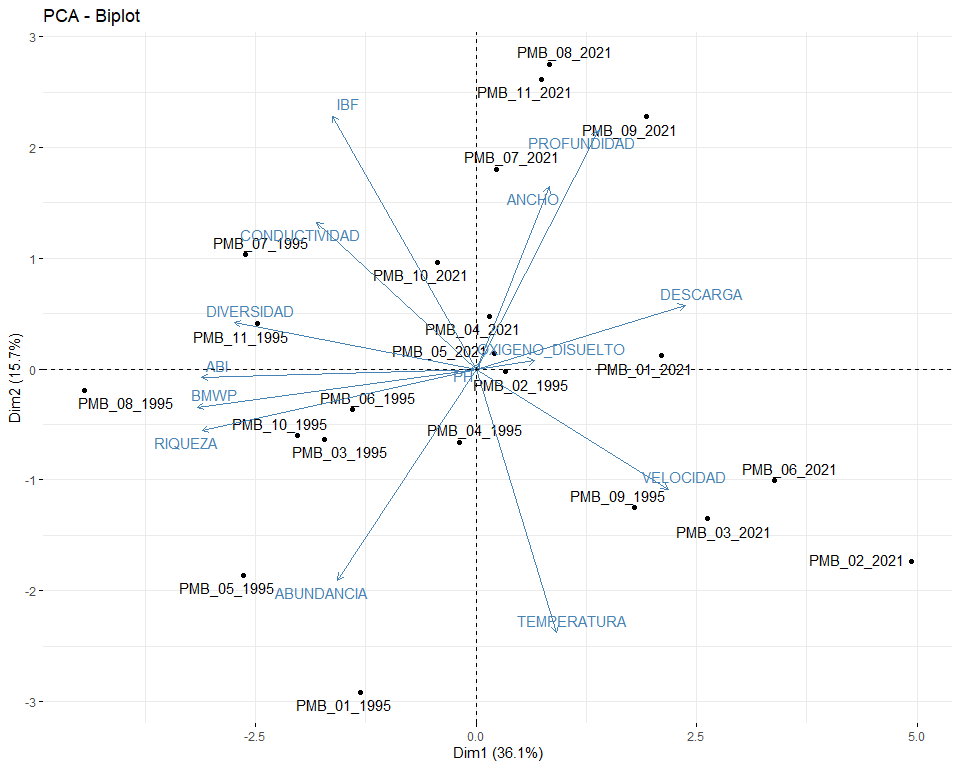
\includegraphics{CaracterizacionEcologica_files/figure-pdf/biplot-1.png}

}

\end{figure}

\begin{quote}
Variables ecológicas como \textbf{ABI, BMWP y RIQUEZA} exhiben una alta
similitud en la estación de monitoreo 8 durante el año 1995. De manera
similar: \textbf{CONDUCTIVIDAD, DIVERSIDAD e IBF} comparten
características destacadas en las estaciones de monitoreo 7 y 11,
también en el año 1995. Por otro lado, un conjunto distinto de variables
como: \textbf{ANCHO, PROFUNDIDAD y DESCARGA} para el año 2021,
evidencian patrones similares en las estaciones de monitoreo 1, 7, 8 y
9. Sin embargo, variables como: \textbf{ABUNDANCIA, TEMPERATURA y
VELOCIDAD}, a pesar de su comportamiento de no similaridad entre ellas,
aportan de forma significativa al modelo factorial individualmente
\end{quote}

\hypertarget{uxedndice-multivariante}{%
\chapter{Índice Multivariante:}\label{uxedndice-multivariante}}

Para la construcción de un \textbf{Índice Multivariante} utilizando el
método factorial por componentes principales, vamos a basarnos en la
utilización de las cargas factoriales o loadings que son los vectores
propios resulantes de la rotación de máxima varianza en las 5
componentes donde se explica el 83\% de variabilidad de los datos,
considerando dos directrices técnicas importantes:

\begin{enumerate}
\def\labelenumi{\arabic{enumi}.}
\tightlist
\item
  Evaluaremos el valor absoluto de las cargas factoriales o loadings
\item
  Estableceremos un umbral mínimo de contribución por variable del 10\%,
  y
\item
  Seleccionaremos, para cada variable y componente, la contribución más
  alta
\end{enumerate}

\begin{Shaded}
\begin{Highlighting}[numbers=left,,]
\FunctionTok{round}\NormalTok{(}\FunctionTok{abs}\NormalTok{((pca}\SpecialCharTok{$}\NormalTok{rotation }\SpecialCharTok{*}\NormalTok{ (pca}\SpecialCharTok{$}\NormalTok{rotation }\SpecialCharTok{\textgreater{}} \SpecialCharTok{{-}}\FloatTok{0.1}\NormalTok{))[, }\DecValTok{1}\SpecialCharTok{:}\DecValTok{5}\NormalTok{]), }\DecValTok{2}\NormalTok{)}
\end{Highlighting}
\end{Shaded}

\begin{verbatim}
                  PC1  PC2  PC3  PC4  PC5
ANCHO            0.08 0.43 0.00 0.04 0.36
PROFUNDIDAD      0.18 0.42 0.05 0.00 0.00
VELOCIDAD        0.30 0.00 0.00 0.00 0.00
DESCARGA         0.31 0.19 0.00 0.01 0.00
PH               0.00 0.05 0.00 0.00 0.01
TEMPERATURA      0.11 0.00 0.00 0.24 0.15
OXIGENO_DISUELTO 0.09 0.00 0.23 0.00 0.25
CONDUCTIVIDAD    0.00 0.26 0.08 0.00 0.13
RIQUEZA          0.00 0.10 0.00 0.04 0.00
ABUNDANCIA       0.00 0.00 0.00 0.07 0.26
DIVERSIDAD       0.00 0.25 0.00 0.04 0.18
ABI              0.00 0.02 0.05 0.00 0.00
BMWP             0.00 0.08 0.04 0.05 0.00
IBF              0.00 0.45 0.00 0.31 0.09
\end{verbatim}

Por consiguiente, la ecuación de las combinaciones lineales para la
matriz de indicadores físico-químicos y ecológicos es la siguiente:

\[\begin{array}{l}{{Y_{1}={\bf a}_{1}X=\ a_{11}X_{1}+a_{12}X_{2}+\cdots+a_{1p}X_{p}}}\\ {{Y_{2}={\bf a}_{21}^{\dagger}X_{1}+\ a_{22}X_{2}+\cdots+a_{2p}X_{p}}}\\ {{\vdots}}\\ {{Y_{p}={\bf a}_{p1}^{\prime}X_{1}+a_{p2}X_{2}+\cdots+a_{p p}X_{p}}}\end{array}\]
Donde:

\(a_{i}:\) Cargas factoriales para cada componente

\(Y_{i}:\) Variables

\hypertarget{ecuaciuxf3n-teuxf3rica}{%
\subsubsection{\texorpdfstring{\textbf{Ecuación
teórica:}}{Ecuación teórica:}}\label{ecuaciuxf3n-teuxf3rica}}

\[I_{mcm} = ANCHO_{\text{PC}2} +\\ PROFUNDIDAD_{\text{PC}2} +\\ VELOCIDAD_{\text{PC}1} +\\ DESCARGA_{\text{PC}1} +\\ PH_{\text{PC}2} +\\ TEMPERATURA_{\text{PC}4} +\\ OXIGENO\_DISUELTO_{\text{PC}5} +\\ CONDUCTIVIDAD_{\text{PC}2} +\\ RIQUEZA_{\text{PC}2} +\\ ABUNDANCIA_{\text{PC}5} +\\ DIVERSIDAD_{\text{PC}2} +\\ ABI_{\text{PC}3} +\\ BMWP_{\text{PC}2} +\\ IBF_{\text{PC}2}\]

\hypertarget{ecuaciuxf3n-del-uxedndice-multidimensional-de-las-comunidades-de-macroinvertebrados-imcm}{%
\subsubsection{\texorpdfstring{\textbf{Ecuación del Índice
Multidimensional de las Comunidades de Macroinvertebrados
(IMCM):}}{Ecuación del Índice Multidimensional de las Comunidades de Macroinvertebrados (IMCM):}}\label{ecuaciuxf3n-del-uxedndice-multidimensional-de-las-comunidades-de-macroinvertebrados-imcm}}

\[I_{mcm} = 0.43 \times ANCHO_{\text{PC}2} +\\ 042 \times PROFUNDIDAD_{\text{PC}2} +\\ 0.30 \times VELOCIDAD_{\text{PC}1} +\\ 0.31 \times DESCARGA_{\text{PC}1} +\\ 0.05 \times PH_{\text{PC}2} +\\ 0.24 \times TEMPERATURA_{\text{PC}4} +\\ 0.25 \times OXIGENO\_DISUELTO_{\text{PC}5} +\\ 0.26 \times CONDUCTIVIDAD_{\text{PC}2} +\\ 0.10 \times RIQUEZA_{\text{PC}2} +\\ 0.26 \times ABUNDANCIA_{\text{PC}5} +\\ 0.25 \times DIVERSIDAD_{\text{PC}2} +\\ 0.05 \times ABI_{\text{PC}3} +\\ 0.08 \times BMWP_{\text{PC}2} +\\ 0.45 \times IBF_{\text{PC}2}\]

\begin{Shaded}
\begin{Highlighting}[numbers=left,,]
\CommentTok{\# Función de escalamiento entre 0 y 1}
\NormalTok{scale\_values }\OtherTok{\textless{}{-}} \ControlFlowTok{function}\NormalTok{(x) \{}
  \FunctionTok{round}\NormalTok{((x }\SpecialCharTok{{-}} \FunctionTok{min}\NormalTok{(x)) }\SpecialCharTok{/}\NormalTok{ (}\FunctionTok{max}\NormalTok{(x) }\SpecialCharTok{{-}} \FunctionTok{min}\NormalTok{(x)),}\DecValTok{2}\NormalTok{)}
\NormalTok{\}}

\NormalTok{indices\_mcm }\OtherTok{\textless{}{-}}\NormalTok{ indices\_fq\_ddc }\SpecialCharTok{\%\textgreater{}\%}
  \FunctionTok{mutate}\NormalTok{(}
    \AttributeTok{INDICE =} \FunctionTok{round}\NormalTok{(}
      \FloatTok{0.43} \SpecialCharTok{*}\NormalTok{ ANCHO }\SpecialCharTok{+}
      \FloatTok{0.42} \SpecialCharTok{*}\NormalTok{ PROFUNDIDAD }\SpecialCharTok{+}
      \FloatTok{0.30} \SpecialCharTok{*}\NormalTok{ VELOCIDAD }\SpecialCharTok{+}
      \FloatTok{0.31} \SpecialCharTok{*}\NormalTok{ DESCARGA }\SpecialCharTok{+}
      \FloatTok{0.05} \SpecialCharTok{*}\NormalTok{ PH }\SpecialCharTok{+}
      \FloatTok{0.24} \SpecialCharTok{*}\NormalTok{ TEMPERATURA }\SpecialCharTok{+}
      \FloatTok{0.25} \SpecialCharTok{*}\NormalTok{ OXIGENO\_DISUELTO }\SpecialCharTok{+}
      \FloatTok{0.26} \SpecialCharTok{*}\NormalTok{ CONDUCTIVIDAD }\SpecialCharTok{+}
      \FloatTok{0.10} \SpecialCharTok{*}\NormalTok{ RIQUEZA }\SpecialCharTok{+}
      \FloatTok{0.26} \SpecialCharTok{*}\NormalTok{ ABUNDANCIA }\SpecialCharTok{+}
      \FloatTok{0.25} \SpecialCharTok{*}\NormalTok{ DIVERSIDAD }\SpecialCharTok{+}
      \FloatTok{0.05} \SpecialCharTok{*}\NormalTok{ ABI }\SpecialCharTok{+}
      \FloatTok{0.08} \SpecialCharTok{*}\NormalTok{ BMWP }\SpecialCharTok{+}
      \FloatTok{0.45} \SpecialCharTok{*}\NormalTok{ IBF, }\DecValTok{2}\NormalTok{),}
    \AttributeTok{IMCM =}  \FunctionTok{scale\_values}\NormalTok{(INDICE),}
    \AttributeTok{RIOS =} \FunctionTok{row.names}\NormalTok{(indices\_fq\_ddc)) }\SpecialCharTok{\%\textgreater{}\%} 
  \FunctionTok{arrange}\NormalTok{(}\FunctionTok{desc}\NormalTok{(IMCM))}

\CommentTok{\# Categorización del I\_MCM con etiquetas personalizadas}
\NormalTok{indices\_mcm}\SpecialCharTok{$}\NormalTok{IMCM\_CATEGORIA }\OtherTok{\textless{}{-}} \FunctionTok{cut}\NormalTok{(indices\_mcm}\SpecialCharTok{$}\NormalTok{IMCM,}
                                  \AttributeTok{breaks =} \FunctionTok{c}\NormalTok{(}\SpecialCharTok{{-}}\ConstantTok{Inf}\NormalTok{, }
                                             \FloatTok{0.29}\NormalTok{,}
                                             \FloatTok{0.30}\NormalTok{,}
                                             \FloatTok{0.49}\NormalTok{,}
                                             \FloatTok{0.62}\NormalTok{,}
                                             \ConstantTok{Inf}\NormalTok{),  }\CommentTok{\# Definición de intervalos}
                                  \AttributeTok{labels =} \FunctionTok{c}\NormalTok{(}\StringTok{"IMCM Bajo"}\NormalTok{,}
                                             \StringTok{"IMCM Bajo"}\NormalTok{,}
                                             \StringTok{"IMCM Medio"}\NormalTok{, }
                                             \StringTok{"IMCM Medio"}\NormalTok{, }
                                             \StringTok{"IMCM Alto"}\NormalTok{),}
                                  \AttributeTok{right =} \ConstantTok{FALSE}\NormalTok{)}

\NormalTok{DT}\SpecialCharTok{::}\FunctionTok{datatable}\NormalTok{(indices\_mcm,}
              \AttributeTok{class =} \StringTok{\textquotesingle{}cell{-}border stripe\textquotesingle{}}\NormalTok{,}
              \CommentTok{\# filter = \textquotesingle{}top\textquotesingle{},}
              \AttributeTok{caption =}\NormalTok{ htmltools}\SpecialCharTok{::}\NormalTok{tags}\SpecialCharTok{$}\FunctionTok{caption}\NormalTok{(}
              \AttributeTok{style =} \StringTok{\textquotesingle{}caption{-}side: bottom; text{-}align: left;\textquotesingle{}}\NormalTok{,}
              \StringTok{\textquotesingle{}Tabla 2: \textquotesingle{}}\NormalTok{, htmltools}\SpecialCharTok{::}\FunctionTok{em}\NormalTok{(}\StringTok{\textquotesingle{}Indicadores Físico{-}Químicos y Ecológicos para los años 1995 y 2021 con el cálculo del Índice Multidimensional de las Comunidades de Macroinvertebrados (IMCM)\textquotesingle{}}\NormalTok{)),}
              \AttributeTok{extensions =} \FunctionTok{c}\NormalTok{(}\StringTok{\textquotesingle{}Buttons\textquotesingle{}}\NormalTok{,}\StringTok{\textquotesingle{}Scroller\textquotesingle{}}\NormalTok{),}
              \AttributeTok{options =} \FunctionTok{list}\NormalTok{(}\AttributeTok{scrollX =} \ConstantTok{TRUE}\NormalTok{,}
                             \AttributeTok{initComplete =} \FunctionTok{JS}\NormalTok{(}
    \StringTok{"function(settings, json) \{"}\NormalTok{,}
    \StringTok{"$(this.api().table().header()).css(\{\textquotesingle{}background{-}color\textquotesingle{}: \textquotesingle{}\#000\textquotesingle{}, \textquotesingle{}color\textquotesingle{}: \textquotesingle{}\#fff\textquotesingle{}\});"}\NormalTok{,}
    \StringTok{"\}"}\NormalTok{),}
    \AttributeTok{dom =} \StringTok{\textquotesingle{}Bfrtip\textquotesingle{}}\NormalTok{,}
    \AttributeTok{buttons =} \FunctionTok{c}\NormalTok{(}\StringTok{\textquotesingle{}excel\textquotesingle{}}\NormalTok{),}
    \AttributeTok{deferRender =} \ConstantTok{TRUE}\NormalTok{,}
    \AttributeTok{scrollY =} \DecValTok{500}\NormalTok{,}
    \AttributeTok{scroller =} \ConstantTok{TRUE}\NormalTok{))}
\end{Highlighting}
\end{Shaded}

\hypertarget{comportamiento-del-imcm-en-los-auxf1os-1995-y-2021}{%
\section{Comportamiento del IMCM en los años 1995 y
2021:}\label{comportamiento-del-imcm-en-los-auxf1os-1995-y-2021}}

\begin{Shaded}
\begin{Highlighting}[numbers=left,,]
\FunctionTok{highchart}\NormalTok{() }\SpecialCharTok{\%\textgreater{}\%}
    \FunctionTok{hc\_chart}\NormalTok{(}\AttributeTok{type =} \StringTok{"column"}\NormalTok{,}
             \AttributeTok{options3d =} \FunctionTok{list}\NormalTok{(}\AttributeTok{enabled =} \ConstantTok{TRUE}\NormalTok{, }
                              \AttributeTok{beta =} \DecValTok{15}\NormalTok{,}
                              \AttributeTok{alpha =} \DecValTok{15}\NormalTok{)) }\SpecialCharTok{\%\textgreater{}\%}  \CommentTok{\# Tipo de gráfico: columnas}
    \FunctionTok{hc\_xAxis}\NormalTok{(}\AttributeTok{categories =}\NormalTok{ indices\_mcm}\SpecialCharTok{$}\NormalTok{RIOS) }\SpecialCharTok{\%\textgreater{}\%}  \CommentTok{\# Especificar las categorías en el eje X}
    \FunctionTok{hc\_add\_series}\NormalTok{(}\AttributeTok{data =}\NormalTok{ indices\_mcm}\SpecialCharTok{$}\NormalTok{IMCM, }
                  \AttributeTok{color =} \StringTok{"\#6096ba"}\NormalTok{) }\SpecialCharTok{\%\textgreater{}\%} 
    \FunctionTok{hc\_xAxis}\NormalTok{(}\AttributeTok{labels =} \FunctionTok{list}\NormalTok{(}\AttributeTok{rotation =} \SpecialCharTok{{-}}\DecValTok{45}\NormalTok{,}
                           \AttributeTok{align =} \StringTok{"right"}\NormalTok{),}
             \AttributeTok{margin =} \DecValTok{100}\NormalTok{) }\SpecialCharTok{\%\textgreater{}\%}
    \FunctionTok{hc\_title}\NormalTok{(}\AttributeTok{text =} \StringTok{"Índice Multidimensional de las Comunidades de Macroinvertebrados por Estaciones de Monitoreo"}\NormalTok{) }\SpecialCharTok{\%\textgreater{}\%}
    \FunctionTok{hc\_caption}\NormalTok{(}\AttributeTok{text =} \StringTok{"Elaborado por: Karina Hernández"}\NormalTok{) }\SpecialCharTok{\%\textgreater{}\%}
    \FunctionTok{hc\_legend}\NormalTok{(}\AttributeTok{enabled =} \ConstantTok{FALSE}\NormalTok{) }\SpecialCharTok{\%\textgreater{}\%}
    \FunctionTok{hc\_tooltip}\NormalTok{(}\AttributeTok{formatter =} \FunctionTok{JS}\NormalTok{(}\StringTok{"function() \{}
\StringTok{                             return \textquotesingle{}\textless{}b\textgreater{}RÍO: \textless{}/b\textgreater{}\textquotesingle{} + this.x + \textquotesingle{}\textless{}br/\textgreater{}\textquotesingle{} +}
\StringTok{                                    \textquotesingle{}\textless{}b\textgreater{}IMCM: \textless{}/b\textgreater{}\textquotesingle{} + this.y.toFixed(2);\}"}\NormalTok{)) }\SpecialCharTok{\%\textgreater{}\%}
    \FunctionTok{hc\_add\_theme}\NormalTok{(}\FunctionTok{hc\_theme\_google}\NormalTok{())}
\end{Highlighting}
\end{Shaded}

\hypertarget{cluxfastering-de-las-estaciones-de-monitoreo-ruxedos}{%
\chapter{Clústering de las estaciones de monitoreo
(Ríos):}\label{cluxfastering-de-las-estaciones-de-monitoreo-ruxedos}}

Para los clusterización de las estaciones de monitoreo se empleará un
método \textbf{No Paramétrico} que se encuentra dentro de los métodos de
\textbf{Aprendizaje No Supervisado}, esto dado porque no se está
utilizando una variable en específico que nos permita clasificar para
entrenar un modelo factorial.

En el proceso de cluster para las estaciones de monitoreo, se utiliza la
misma estructura matricial de los índices físico-químicos y ecológicos.
Por consiguiente se utiliza el siguiente proceso algorítmico:

\begin{enumerate}
\def\labelenumi{\arabic{enumi}.}
\tightlist
\item
  Definición del número óptimo de clústers
\item
  Algoritmo K-Means
\end{enumerate}

\hypertarget{escalamiento-de-la-matriz-de-datos-y-elecciuxf3n-del-nuxfamero-uxf3ptimo-de-cluxfasters}{%
\section{Escalamiento de la matriz de datos y elección del número óptimo
de
clústers:}\label{escalamiento-de-la-matriz-de-datos-y-elecciuxf3n-del-nuxfamero-uxf3ptimo-de-cluxfasters}}

\begin{Shaded}
\begin{Highlighting}[numbers=left,,]
\NormalTok{var\_scale }\OtherTok{\textless{}{-}} \FunctionTok{as.data.frame}\NormalTok{(}\FunctionTok{lapply}\NormalTok{(indices\_fq\_ddc, }\ControlFlowTok{function}\NormalTok{(x) }\ControlFlowTok{if}\NormalTok{(}\FunctionTok{is.numeric}\NormalTok{(x)) }\FunctionTok{scale}\NormalTok{(x) }\ControlFlowTok{else}\NormalTok{ x))}

\NormalTok{algoritmo }\OtherTok{\textless{}{-}} \FunctionTok{kmeans}\NormalTok{(var\_scale,}
             \AttributeTok{centers =} \DecValTok{4}\NormalTok{,}
             \AttributeTok{algorithm =} \StringTok{"Hartigan{-}Wong"}\NormalTok{,}
             \AttributeTok{iter.max =} \DecValTok{100}\NormalTok{) }\CommentTok{\#se cambia center por el numero de cluster}
\end{Highlighting}
\end{Shaded}

\hypertarget{muxe9todo-del-codo}{%
\section{Método del codo:}\label{muxe9todo-del-codo}}

\begin{Shaded}
\begin{Highlighting}[numbers=left,,]
\FunctionTok{fviz\_nbclust}\NormalTok{(var\_scale,}
\NormalTok{             kmeans, }
             \AttributeTok{method =} \StringTok{"wss"}\NormalTok{) }\SpecialCharTok{+}
  \FunctionTok{labs}\NormalTok{(}\AttributeTok{subtitle =} \StringTok{"Elbow Method"}\NormalTok{) }\SpecialCharTok{+}
  \FunctionTok{geom\_vline}\NormalTok{(}\AttributeTok{xintercept =} \DecValTok{4}\NormalTok{)}
\end{Highlighting}
\end{Shaded}

\begin{figure}[tb]

{\centering \includegraphics{CaracterizacionEcologica_files/figure-pdf/unnamed-chunk-2-1.png}

}

\end{figure}

\hypertarget{conformaciuxf3n-de-cluxfasters}{%
\section{Conformación de
clústers:}\label{conformaciuxf3n-de-cluxfasters}}

\begin{Shaded}
\begin{Highlighting}[numbers=left,,]
\FunctionTok{fviz\_cluster}\NormalTok{(algoritmo,}
             \AttributeTok{data =}\NormalTok{ var\_scale) }\SpecialCharTok{+}
    \FunctionTok{theme\_minimal}\NormalTok{() }\SpecialCharTok{+}
    \FunctionTok{labs}\NormalTok{(}
        \AttributeTok{title =} \StringTok{"Clústers de las Estaciones de Monitoreo"}\NormalTok{,}
        \AttributeTok{caption =} \StringTok{"Elaborado por: Karina Hernández"}\NormalTok{) }\SpecialCharTok{+}
    \FunctionTok{theme\_minimal}\NormalTok{() }\SpecialCharTok{+}
    \FunctionTok{theme}\NormalTok{(}
        \AttributeTok{axis.text.x =} \FunctionTok{element\_text}\NormalTok{(}\AttributeTok{angle =} \DecValTok{0}\NormalTok{,}
                                   \AttributeTok{vjust =} \FloatTok{0.5}\NormalTok{,}
                                   \AttributeTok{hjust =} \FloatTok{0.5}\NormalTok{),}
        \AttributeTok{axis.title.x =} \FunctionTok{element\_text}\NormalTok{(}\AttributeTok{angle =} \DecValTok{0}\NormalTok{),}
        \AttributeTok{axis.title.y =} \FunctionTok{element\_text}\NormalTok{(}\AttributeTok{angle =} \DecValTok{0}\NormalTok{),}
        \AttributeTok{panel.grid =} \FunctionTok{element\_line}\NormalTok{(}\AttributeTok{color =} \StringTok{"\#e9ecef"}\NormalTok{, }\AttributeTok{linewidth =} \FloatTok{0.5}\NormalTok{),  }\CommentTok{\# Cambio a linewidth}
        \AttributeTok{panel.border =} \FunctionTok{element\_rect}\NormalTok{(}\AttributeTok{color =} \StringTok{"black"}\NormalTok{, }\AttributeTok{fill =} \ConstantTok{NA}\NormalTok{),}
        \AttributeTok{axis.ticks =} \FunctionTok{element\_line}\NormalTok{(}\AttributeTok{color =} \StringTok{"black"}\NormalTok{),}
        \AttributeTok{axis.line =} \FunctionTok{element\_blank}\NormalTok{(),}
        \AttributeTok{plot.title =} \FunctionTok{element\_text}\NormalTok{(}\AttributeTok{hjust =} \FloatTok{0.5}\NormalTok{),}
        \AttributeTok{plot.caption =} \FunctionTok{element\_text}\NormalTok{(}\AttributeTok{hjust =} \DecValTok{0}\NormalTok{),}
        \AttributeTok{axis.ticks.length =} \FunctionTok{unit}\NormalTok{(}\SpecialCharTok{{-}}\FloatTok{0.1}\NormalTok{, }\StringTok{"cm"}\NormalTok{))}
\end{Highlighting}
\end{Shaded}

\begin{figure}[tb]

{\centering \includegraphics{CaracterizacionEcologica_files/figure-pdf/unnamed-chunk-3-1.png}

}

\end{figure}

\hypertarget{tabla-final}{%
\section{Tabla final:}\label{tabla-final}}

\begin{Shaded}
\begin{Highlighting}[numbers=left,,]
\NormalTok{indices\_mcm }\OtherTok{\textless{}{-}}\NormalTok{ indices\_mcm }\SpecialCharTok{\%\textgreater{}\%}
  \FunctionTok{mutate}\NormalTok{(}\AttributeTok{CLUSTER =} \FunctionTok{as.factor}\NormalTok{(algoritmo}\SpecialCharTok{$}\NormalTok{cluster))}

\NormalTok{DT}\SpecialCharTok{::}\FunctionTok{datatable}\NormalTok{(indices\_mcm,}
              \AttributeTok{class =} \StringTok{\textquotesingle{}cell{-}border stripe\textquotesingle{}}\NormalTok{,}
              \CommentTok{\# filter = \textquotesingle{}top\textquotesingle{},}
              \AttributeTok{caption =}\NormalTok{ htmltools}\SpecialCharTok{::}\NormalTok{tags}\SpecialCharTok{$}\FunctionTok{caption}\NormalTok{(}
              \AttributeTok{style =} \StringTok{\textquotesingle{}caption{-}side: bottom; text{-}align: left;\textquotesingle{}}\NormalTok{,}
              \StringTok{\textquotesingle{}Tabla 3: \textquotesingle{}}\NormalTok{, htmltools}\SpecialCharTok{::}\FunctionTok{em}\NormalTok{(}\StringTok{\textquotesingle{}Indicadores Físico{-}Químicos y Ecológicos para los años 1995 y 2021 con el cálculo del Índice Multidimensional de las Comunidades de Macroinvertebrados (IMCM) y el número de clúster que corresponde\textquotesingle{}}\NormalTok{)),}
              \AttributeTok{extensions =} \FunctionTok{c}\NormalTok{(}\StringTok{\textquotesingle{}Buttons\textquotesingle{}}\NormalTok{,}\StringTok{\textquotesingle{}Scroller\textquotesingle{}}\NormalTok{),}
              \AttributeTok{options =} \FunctionTok{list}\NormalTok{(}\AttributeTok{scrollX =} \ConstantTok{TRUE}\NormalTok{,}
                             \AttributeTok{initComplete =} \FunctionTok{JS}\NormalTok{(}
    \StringTok{"function(settings, json) \{"}\NormalTok{,}
    \StringTok{"$(this.api().table().header()).css(\{\textquotesingle{}background{-}color\textquotesingle{}: \textquotesingle{}\#000\textquotesingle{}, \textquotesingle{}color\textquotesingle{}: \textquotesingle{}\#fff\textquotesingle{}\});"}\NormalTok{,}
    \StringTok{"\}"}\NormalTok{),}
    \AttributeTok{dom =} \StringTok{\textquotesingle{}Bfrtip\textquotesingle{}}\NormalTok{,}
    \AttributeTok{buttons =} \FunctionTok{c}\NormalTok{(}\StringTok{\textquotesingle{}excel\textquotesingle{}}\NormalTok{),}
    \AttributeTok{deferRender =} \ConstantTok{TRUE}\NormalTok{,}
    \AttributeTok{scrollY =} \DecValTok{500}\NormalTok{,}
    \AttributeTok{scroller =} \ConstantTok{TRUE}\NormalTok{))}
\end{Highlighting}
\end{Shaded}

\hypertarget{flujo-del-modelo-factorial}{%
\subsection{Flujo del Modelo
Factorial}\label{flujo-del-modelo-factorial}}

\begin{Shaded}
\begin{Highlighting}[numbers=left,,]
\NormalTok{graph TD;}
\NormalTok{    A(Matriz de correlaciones y su significancia estadística) {-}{-}\textgreater{} }
\NormalTok{    B(Determinante de la matriz de correlaciones);}
\NormalTok{    B {-}{-}\textgreater{} C(Prueba de esfericidad de Bartlett);}
\NormalTok{    C {-}{-}\textgreater{} D(Comprobación de hipótesis para el análisis factorial por componentes principales);}
\NormalTok{    D {-}{-}\textgreater{} E(Gráfico de Sedimentación);}
\NormalTok{    E {-}{-}\textgreater{} F(Proporción de Varianza Acumulada);}
\NormalTok{    F {-}{-}\textgreater{} G(Componentes Principales);}
\NormalTok{    G {-}{-}\textgreater{} H(Autovalores y Varianzas);}
\NormalTok{    H {-}{-}\textgreater{} I(Círculo de las Correlaciones);}
\NormalTok{    I {-}{-}\textgreater{} J(Variables versus Dimensiones);}
\NormalTok{    J {-}{-}\textgreater{} K(Biplot);}
\end{Highlighting}
\end{Shaded}

\begin{figure}[H]

{\centering \includegraphics[width=6.44in,height=9.84in]{CaracterizacionEcologica_files/figure-latex/mermaid-figure-1.png}

}

\end{figure}


\printbibliography[title=Bibliografía]


\end{document}
